%=================================================================
%  PeerJ (PeerJ Inc. / Taylor & Francis). wlpeerj class.
%  Build: pdflatex x2, bibtex, pdflatex x2. Line numbers on for review.
%=================================================================
\documentclass[fleqn,10pt,lineno]{wlpeerj}
\usepackage{siunitx}
\usepackage{textcomp}
\DeclareMathSymbol{-}{\mathbin}{operators}{"2D}
\usepackage[hidelinks]{hyperref}
\usepackage{url}
\usepackage{xurl}
\usepackage{amsmath}
\usepackage{booktabs}
\usepackage{graphicx}
\emergencystretch=3em
\sloppy
\providecommand{\doi}[1]{\href{https://doi.org/#1}{\nolinkurl{#1}}}

\graphicspath{{figures/}}

%% Front-matter macros, defined here rather than taken from a journal class: this
%% source carries no venue, and convert_to_peerj.py rebuilds the title block for
%% PeerJ. The definitions below are minimal no-ops except where they must retain a
%% value, so the body compiles unchanged.
%% \abstract is an environment in the article class, so it is only redefined if the
%% class did not already define it as a command.
%% Back-matter declaration commands. convert_to_peerj.py reads these by name and
%% rebuilds the PeerJ declarations block, so they only have to retain their argument.

\newcommand{\nFirst}{41}
\newcommand{\nLast}{706}
\newcommand{\growth}{17.2}
%% Archive inventory, read from UO_ARCHIVE_MANIFEST.json, which is committed and
%% pins every archive member by byte count and SHA-256. The manifest matches the
%% local archive and the deposited snapshot exactly: 884 members, 73.8 GB (decimal,
%% as \giga\byte prints; the same quantity is 68.7 GiB).
%%
%% These three were previously hardcoded as 882 files / 68 GB and had drifted three
%% files behind the archive, and the prose sentence "the 882 is their sum" did not
%% even equal the per-year counts it lists (which sum to 881 without this fix).
%% verify_paper_numbers.py now recomputes them from the manifest, so they gate CI.
\newcommand{\nArchiveFiles}{884}
\newcommand{\nArchiveGB}{73.8}
%% TOTAL readings across the whole archive, 2013--2026, counted directly from every
%% CSV in every UO-archive-YYYY.zip (data rows = lines - 1 per file, one header row).
%% Method validated against Python's csv.reader on all eight themes (lines == records)
%% and the 2026 archive hash-checked against UO_ARCHIVE_MANIFEST.json (sha256 identical).
%%
%% WHY THIS REPLACES A HARDCODED NUMBER. The prose used to read "155 million readings
%% in the 2026 year alone", a bare integer typed into the text. It was wrong twice over:
%% measured 2026 is 176,254,027 (the claim was 88% of it), AND 2026 is not the largest
%% year -- it ranks 10th of 14 at 36% of 2023. The year chosen to illustrate the
%% archive's scale was among its smaller recent years. The total is used instead because
%% it needs no ranking of years, which is the error the claim made.
%%
%% Per-year counts, for reference:
%%   2013 4,244,933 | 2014 8,371,091 | 2015 27,120,328 | 2016 175,377,835
%%   2017 310,631,407 | 2018 309,802,130 | 2019 428,075,479 | 2020 468,184,233
%%   2021 381,566,067 | 2022 372,547,165 | 2023 489,784,193 | 2024 261,525,899
%%   2025 209,368,033 | 2026 176,254,027  (partial: nine months)
\newcommand{\nArchiveReadings}{3622852820}
%% 2026 is the partial year; LaTeX control sequences cannot contain digits, so
%% this is \nFilesLast rather than \nFiles2026.
\newcommand{\nFilesLast}{257}
\newcommand{\rFirst}{0.729}
\newcommand{\rLast}{0.238}
\newcommand{\rDrop}{67}
%% R on each year's own hull. Support matching ENLARGES the decline (64.7% against 45% on the
%% fixed hull), because a small early footprint raises the early R. The paper previously called
%% the fixed-hull figure an "upper bound"; that is backwards and is corrected here.
\newcommand{\rOwnHull}{64.7}
\newcommand{\rOwnHullFirst}{0.942}
\newcommand{\rOwnHullLast}{0.332}
\newcommand{\locFirst}{0.751}
\newcommand{\locLast}{0.309}
\newcommand{\rSlope}{-0.031}
\newcommand{\rSlopeLO}{-0.042}
\newcommand{\rSlopeHI}{-0.019}
\newcommand{\plSlope}{-0.369}
\newcommand{\plLO}{-0.534}
\newcommand{\plHI}{-0.311}
\newcommand{\plRtwo}{0.849}
\newcommand{\giniRareP}{0.04}
\newcommand{\giniRareSlope}{-0.004}
\newcommand{\giniRareLO}{-0.008}
\newcommand{\giniRareHI}{-0.001}
\newcommand{\giniRawSlope}{0.013}
\newcommand{\giniRareTrend}{0.45}
\newcommand{\covPct}{64.9}
\newcommand{\omitN}{667}
\newcommand{\omitVeh}{63.1}
% --- round-five figures, all from results_churn.json ---
\newcommand{\growthLoc}{14.4}
\newcommand{\dropNt}{39}
\newcommand{\plateauLocSlope}{+0.000}
\newcommand{\plateauLocRtwo}{0.000}
\newcommand{\plateauIdSlope}{-0.010}
\newcommand{\replMedian}{0.58}
\newcommand{\vehOR}{0.45}
\newcommand{\actCovPct}{66.5}
\newcommand{\giniIntSlope}{-0.003}
\newcommand{\giniIntLO}{-0.007}
\newcommand{\giniIntHI}{+0.000}
\newcommand{\giniIntLOtwo}{-0.006}
\newcommand{\giniIntHItwo}{+0.003}
\newcommand{\giniIntSlopeTwo}{-0.002}
\newcommand{\rRareSlope}{\mbox{$\approx$0}}
\newcommand{\rRareLO}{-0.005}
\newcommand{\rRareHI}{+0.005}
% --- round-eight figures, results_theilsen.json ---
% Theil-Sen intervals recomputed correctly: the slope is the median of the
% pairwise slopes and the interval is the rank-based interval for that median,
% NOT the spread of the pairwise slopes. Values from analysis_theilsen.py.
\newcommand{\rRareTS}{-0.000}
\newcommand{\rRareTSLO}{-0.005}
\newcommand{\rRareTSHI}{+0.006}
\newcommand{\gRareTS}{-0.005}
\newcommand{\gRareTSLO}{-0.009}
\newcommand{\gRareTSHI}{-0.001}
\newcommand{\rHullLocTS}{-0.010}
\newcommand{\rHullLocTSLO}{-0.022}
\newcommand{\rHullLocTSHI}{-0.005}
\newcommand{\rHullTS}{-0.015}
\newcommand{\rHullTSLO}{-0.028}
\newcommand{\rHullTSHI}{-0.005}
\newcommand{\boxTS}{-0.028}
\newcommand{\boxTSLO}{-0.040}
\newcommand{\boxTSHI}{-0.019}
% minimum detectable effect for the rarefied null (replaces post-hoc power)
% computed in analysis_rarefy.py; recomputed at the stated SE and df, 2026-10-01
\newcommand{\rRareMDE}{0.008}
\newcommand{\rRareMDEtwo}{0.010}
% --- round-fifteen: CSR envelope over 199 realisations at three sizes ---
% results_envelope.json. The control is a DRAW, not a closed form, so it
% carries sampling scatter; the residual is the bias of the estimator itself.
\newcommand{\envN}{199}
\newcommand{\envBiasLast}{4.1}
\newcommand{\envScatterLast}{50}
\newcommand{\envBiasFirst}{262.7}
\newcommand{\envScatterFirst}{565.6}
\newcommand{\envBiasMid}{33.3}
\newcommand{\envScatterMid}{139.9}
\newcommand{\envBiasMinPct}{3.4}
\newcommand{\envBiasMaxPct}{13.5}
% leave-one-out intensity: a local Clark--Evans ratio d_i / (1/(2 sqrt(lam_i))) where lam_i is
% the kernel intensity at x_i fitted WITHOUT x_i (h = 750 m). Below 1 means the point's nearest
% neighbour is closer than its own leave-one-out local density predicts, i.e. local clustering.
% NB: TeX control sequences take LETTERS ONLY, so these must not contain digits.
\newcommand{\looIntFirst}{1.27}
\newcommand{\looIntMid}{0.25}
\newcommand{\looIntLast}{0.069}
% --- round-fifteen: snapshot provenance detail ---
% results_snapdupes.json. The 179 snapshot-only identifiers resolve by
% nearest census location: most are duplicate registrations, not new sites.
\newcommand{\snapDupWithin}{114}
\newcommand{\snapDupWithinPct}{63.7}
\newcommand{\snapDupMedian}{6.4}
\newcommand{\snapDupLocs}{84}
\newcommand{\snapDupNearPct}{84.9}
\newcommand{\snapDupFar}{27}
\newcommand{\snapVehInPct}{51.4}
\newcommand{\snapVehOmPct}{72.9}
\newcommand{\snapCondOR}{2.55}
\newcommand{\snapCondFisher}{1.64}
\newcommand{\giniMDE}{0.0046}
% comparisons run in total (frames x units x years, resolutions, anchors, ...)
\newcommand{\nComp}{182}
% single random seed used for every draw in the paper (stability checked in §4)
\newcommand{\randSeed}{20261003}
% rarefied clustering on the LOCATION unit (the primary unit), N = 39 locations
\newcommand{\rRareLocSlope}{+0.002}
\newcommand{\rRareLocLO}{-0.002}
\newcommand{\rRareLocHI}{+0.006}
% urban-extent mask (union of 2 km buffers around all locations), fixed frame
\newcommand{\maskArea}{1601}
\newcommand{\maskFirst}{0.610}
\newcommand{\maskLast}{0.335}
\newcommand{\maskRescale}{1.66}
% per-year (support-matched) 2 km mask, a LEVEL comparison only
\newcommand{\pyMaskFirst}{1.55}
\newcommand{\pyMaskLast}{0.46}
\newcommand{\pyMaskAreaMin}{247}
\newcommand{\pyMaskAreaPeak}{1192}
\newcommand{\pyMaskAreaLast}{868}
\newcommand{\pyMaskThreshold}{1.8}
\newcommand{\rRareLocFirst}{0.367}
\newcommand{\rRareLocLast}{0.382}
\newcommand{\rRareLocN}{39}
% fixed-hull slope sensitivity to the discontinuity and the partial year
\newcommand{\hullSensAll}{-0.011}
\newcommand{\hullSensNoDisc}{-0.011}
\newcommand{\hullSensNoLast}{-0.010}
\newcommand{\hullSensBoth}{-0.010}
\newcommand{\gRareSlope}{-0.004}
\newcommand{\gRareLO}{-0.008}
\newcommand{\gRareHI}{-0.001}
\newcommand{\gRareAnchorLO}{-0.007}
\newcommand{\gRareAnchorHI}{+0.000}
\newcommand{\gRareAnchorTwoLO}{-0.006}
\newcommand{\gRareAnchorTwoHI}{+0.003}
% clean regression: ln d_bar on ln N, slope tested against the structural -1/2
% clean ln d-bar ~ ln N regression. The published values are the IDENTIFIER unit; the paper's
% primary unit is locations, which gives -0.603 (analysis_reframe.py)
\newcommand{\cleanSlope}{-0.651}
\newcommand{\cleanLO}{-0.839}
\newcommand{\cleanHI}{-0.463}
\newcommand{\cleanT}{-1.75}
\newcommand{\cleanSlopeLoc}{-0.603}
\newcommand{\cleanSELoc}{0.068}
\newcommand{\cleanTLoc}{-1.52}
\newcommand{\cleanPLoc}{0.15}
\newcommand{\cleanSlopeSite}{-0.550}
\newcommand{\cleanSlopeSiteTwo}{-0.426}
\newcommand{\thinningBeta}{-0.745}
% isotropy: directional K by orientation sector, 8 sectors at 1 km (analysis_reframe.py)
\newcommand{\isoRatio}{1.42}
\newcommand{\isoChi}{81.3}
\newcommand{\isoOutside}{0}
% Rotation null (999 rotations of the observed 2026 pattern about its centroid, inside the
% fixed hull, preserving clustering and pair count). The CSR null previously used here was
% powerless: at n = 561 the envelope spans half to double 1/8 per sector, so 0 of 8 outside
% carried no information. The CSR ratio at the observed n is 2.33 (sd 0.69), not evidence.
\newcommand{\isoRotMean}{1.37}
\newcommand{\isoRotSd}{0.06}
\newcommand{\isoRotOutside}{1}
% Dense CSR inside the same hull isolates the WINDOW's own anisotropy: 1.01, so the window
% does not explain the observed 1.42. This reverses an earlier claim in this paper.
\newcommand{\isoWindowRatio}{1.01}
% --- round-thirteen: correctly sized inference (results_trendtests.json) ---
% The Newey-West t-test with a t(12) critical value is oversized at fourteen points:
% simulated on pure noise it rejects 16.3% of the time at a nominal 5%, 19.3% at AR(1)
% rho=0.15 and 29.4% at rho=0.5, because the Bartlett-weighted autocovariance sum can
% fall below the OLS variance. The plain OLS test is correctly sized in the same
% simulation: an i.i.d. draw rejects at 4.7% and the AR(1) rho=0 cell at 4.9%, both
% consistent with a nominal 5%, so the HAC family is the sensitivity and the primary
% tests are OLS, permutation and Mann-Kendall.
\newcommand{\nwSize}{16.3}
\newcommand{\nwSizeAr}{19.3}
\newcommand{\nwSizeArHigh}{29.4}
\newcommand{\olsSizeIid}{4.7}
\newcommand{\olsSizeAr}{8.5}
\newcommand{\hullLocOlsP}{0.037}
\newcommand{\hullLocPermP}{0.038}
\newcommand{\hullLocMkP}{0.010}
\newcommand{\hullIdsOlsP}{0.018}
\newcommand{\hullNoLastOlsP}{0.095}
\newcommand{\hullNoLastPermP}{0.101}
\newcommand{\hullNoLastMkP}{0.030}
\newcommand{\hullNoDiscMkP}{0.017}
% rarefied Gini robustness: the residual decline does not survive dropping the anchor
\newcommand{\gRareNoAnchorSlope}{-0.003}
\newcommand{\gRareNoAnchorOlsP}{0.246}
\newcommand{\gRareNoAnchorMkP}{0.129}
% --- round-fourteen: edge correction, endpoint, theme composition, gap-filled L ---
% All four edge treatments decline; the border estimator carries its own small bias
% (0.90 on CSR at n=100), so it is a sensitivity and not the headline.
\newcommand{\edgePlain}{-0.011}
\newcommand{\edgeBorder}{-0.013}
\newcommand{\edgeGuard}{-0.012}
\newcommand{\edgePlainP}{0.037}
\newcommand{\edgeBorderP}{0.000}
\newcommand{\epSlope}{-0.010}
\newcommand{\epSlopeP}{0.016}
\newcommand{\epMkP}{0.030}
\newcommand{\vehSlope}{-0.012}
\newcommand{\vehMkP}{0.014}
\newcommand{\gapLPub}{-426}
\newcommand{\gapLFilled}{-371}
% random-labelling infill test: new locations are FARTHER than chance in 12/13.
% 2016 is INSIDE its envelope (observed 232 m against [127, 300]), which an earlier
% version of this paper reported as 13 of 13 by comparing the wrong quantity.
\newcommand{\rlAbove}{12}
\newcommand{\rlInside}{1}
\newcommand{\rlInsideYear}{2016}
\newcommand{\rlPairs}{13}
% batch deployment: new locations are clustered among THEMSELVES, tested against
% random subsets of the pooled set (the random-labelling logic), not against CSR
\newcommand{\batchPairs}{10}
\newcommand{\batchTotal}{13}
% inhomogeneous null bandwidth sensitivity and itemised years
\newcommand{\bwM}{750}
% location-based fixed-hull headline (the primary unit)
\newcommand{\locHullDrop}{45}
% gap-filled population rerun
\newcommand{\gfRSlope}{-0.011}
\newcommand{\gfGiniSlope}{+0.013}
% --- round-six figures, results_inhomogeneous.json and the fixed-region rerun ---
% R on the full-record convex hull, a single geographic reference frame held
% fixed for every year. HAC lag 2.
\newcommand{\rHullFirst}{0.357}
\newcommand{\rHullLast}{0.155}
\newcommand{\rHullDrop}{57}
\newcommand{\rHullSlope}{-0.013}
\newcommand{\rHullLO}{-0.021}
\newcommand{\rHullHI}{-0.004}
\newcommand{\rHullLocFirst}{0.367}
\newcommand{\rHullLocLast}{0.202}
\newcommand{\rHullLocDrop}{45}
\newcommand{\rHullLocSlope}{-0.011}
\newcommand{\rHullLocLO}{-0.019}
\newcommand{\rHullLocHI}{-0.003}
% R with the full-record bounding box as the fixed area (2013 0.294 -> 2026 0.128)
\newcommand{\rFixAreaFirst}{0.294}
\newcommand{\rFixAreaLast}{0.128}
\newcommand{\rFixAreaSlope}{-0.010}
% power law on the fixed hull: the size scaling does NOT survive the fixed window
\newcommand{\plHullSlope}{-0.151}
\newcommand{\plHullLO}{-0.337}
\newcommand{\plHullHI}{+0.036}
\newcommand{\plHullRtwo}{0.164}
% joint fit on the fixed hull: size loses significance, year keeps it
\newcommand{\jhSize}{+0.136}
\newcommand{\jhSizeLO}{-0.127}
\newcommand{\jhSizeHI}{+0.399}
\newcommand{\jhYear}{-0.075}
\newcommand{\jhYearLO}{-0.136}
\newcommand{\jhYearHI}{-0.015}
\newcommand{\jhRtwo}{0.514}
% --- tolerance (near-duplicate) robustness, results_tolerance.json ---
% the sweep: no plateau, so the published tolerance is one rung on a continuum
\newcommand{\tolFallOne}{44.9}
\newcommand{\tolPOne}{0.037}
\newcommand{\tolFallFive}{42.5}
\newcommand{\tolPFive}{0.053}
\newcommand{\tolFallTen}{34.1}
\newcommand{\tolPTen}{0.120}
\newcommand{\tolFallFifteen}{21.1}
\newcommand{\tolPFifteen}{0.359}
\newcommand{\tolFallFifty}{-6.8}
\newcommand{\tolPFifty}{0.320}
% share vs surplus, 2026
\newcommand{\shareTwoFive}{524}
\newcommand{\surplusTwoFive}{306}
\newcommand{\surplusAlready}{145}
% merging robustness
\newcommand{\clFall}{4.7}
\newcommand{\clP}{0.774}
\newcommand{\chainMax}{74}
\newcommand{\chainMedian}{12}
\newcommand{\gridSnapFall}{31.1}
\newcommand{\gridSnapP}{0.146}
% L is not invariant to the merge: 1 km slope under each unit
\newcommand{\lKmExact}{-426}
\newcommand{\lKmExactP}{0.005}
\newcommand{\lKmSitesTen}{-437}
\newcommand{\lKmSitesTwentyFive}{-456}
\newcommand{\lKmSitesTwentyFiveP}{0.003}
\newcommand{\lKmNoThin}{-283}
% NN gap below 200 m, the range that could justify a tolerance
\newcommand{\nnGapMax}{35}
% equivalence and power for the rarefied R null (Section 3.2)
\newcommand{\tostR}{0.001}
\newcommand{\powR}{100}
% Gini over all cells including empty ones (extent-sensitive), slope and interval
\newcommand{\giniAllSlope}{-0.001}
\newcommand{\giniAllLO}{-0.012}
\newcommand{\giniAllHI}{+0.006}
% J-function infill diagnostic: median J at 500 m across the thirteen year pairs
\newcommand{\jMed}{0.42}
% window sizes
\newcommand{\winEW}{66}
\newcommand{\winNS}{98}
% Location-based endpoint fall, measured 2026-09-30: 0.751 -> 0.309 = 58.8%.
% The identifier-based fall is 67.4%. Both are reported because the identifier
% scheme accounts for ~9 points of the difference.
\newcommand{\locDrop}{59}
\newcommand{\births}{1906}
\newcommand{\silences}{1200}
% --- spatial-unit figures, measured 2026-09-29 from the identifier catalogue ---
% 1906 identifiers occur at 1574 distinct coordinates (rounded to 1e-6 degrees);
% 332 of the 1906 share a coordinate with at least one other, and the largest
% co-located group is 10. Co-location per year is small and DECLINING
% (2013 45 ids/43 locs = 4.4%, 2014 111/109 = 1.8%, 2015 380/374 = 1.6%),
% so the unit of analysis cannot drive the clustering trend.
\newcommand{\nIdentifiers}{1906}
\newcommand{\nAnalysed}{1899}
\newcommand{\nLocations}{1567}
\newcommand{\nShared}{599}
\newcommand{\nSurplus}{332}
\newcommand{\sharePct}{31.5}
\newcommand{\surplusPct}{17.5}
\newcommand{\surplusMax}{22.8}
\newcommand{\maxCoLoc}{10}

% Umm Al-Qura University publication-support grant identifier (Path 7:
% Scientific Publication Support), observed as
%   26UQU<7-digit staff number>GSSR<2-digit sequence>
% which is what 26UQU4350624GSSR07 is: a 7-digit staff number, the literal track
% code GSSR (Postgraduate Studies and Scientific Research), and 07.
%
% The two statements differ in attribution BY DESIGN, following UQU's own
% wording:
%   funding  : "This research work was funded by Umm Al-Qura University, Saudi
%               Arabia under grant number: ..."            (the University)
%   thanks   : "The authors would like to thank the Deanship of Postgraduate
%               Studies and Research at Umm Al-Qura University for funding this
%               work under grant number: ..."            (the Deanship)
% The funding statement names the University; the acknowledgement names the
% Deanship that administers the award. Both say "grant number" and carry the
% same value, which is what UQU requires.
%
% The award reimburses the APC after publication, so no fee is paid up front and
% nothing is charged to the authors directly.
\newcommand{\uquGrant}{26UQU4350624GSSR07}



% Author ORCIDs are the authors' own. Ammar Arbaaeen and Ammar Alsaig are at Umm Al-Qura
% University, Department of Computer Science; Wael Alnahari (CORRESPONDING, and NOT the
% first author -- author order and the corresponding-author field are independent) and
% Tawfiq Hasanin are at King Abdulaziz University, Department of Information Systems;
% Wasem Alnahri is an independent researcher.
% is at King Abdulaziz University, Department of Information Systems.











%=================================================================
% Front matter. No venue commands: convert_to_peerj.py rebuilds this block.
%=================================================================











\title{Measurement-Dependent Clustering in the Growing Urban Observatory
Sensor Network}

\author[2]{Ammar Arbaaeen}
\author[1]{Wael Alnahari}
\author[2]{Ammar Alsaig}
\author[1]{Tawfiq Hasanin}
\author[3]{Wasem Alnahri}

\affil[1]{Department of Information Systems, Faculty of Computing and Information Technology, King Abdulaziz University, Jeddah 21589, Saudi Arabia}
\affil[2]{Department of Computer Science, College of Computer and Information Systems, Umm Al-Qura University, Mecca 24381, Saudi Arabia}
\affil[3]{Independent Researcher, Mecca 24331, Saudi Arabia}

\corrauthor[1]{Wael Alnahari}{walnahari0004@stu.kau.edu.sa}

\let\origTheCorrAuthor\thecorrauthor
\def\thecorrauthor{\origTheCorrAuthor\medskip
Postal address: MDFA3058, 3058 Prince Nasser bin Abdulaziz Street, King Fahd District, Makkah 24342, Saudi Arabia\par}

\begin{abstract}
Urban sensing studies describe a network from a single slice, so they cannot show
whether its structure changes as it grows. We census the Newcastle
Urban Observatory instrument population annually, \num{2013}--\num{2026} (\nFirst{} to \nLast{} identifiers), and ask
how much of the apparent strengthening of nearest-neighbour clustering is a property of the
deployment, not the measurement. The Clark--Evans index falls \rDrop\% on each year's
own bounding box and identifiers, \rHullDrop\% on a fixed reference hull, and \locHullDrop\% once
identifiers at one coordinate are counted once; measuring each year on its own hull gives \rOwnHull\%. Merging registrations within \SI{25}{\meter} leaves \num{4.3}\%, shrinking
monotonically with no plateau, so the tolerance is a choice, not a threshold the data identify.
The two controls interact rather than partition the decline: registration removes it on the fixed
hull, support matching restores \num{38.6}\%, so we report a range, not a decomposition. On each
year's own footprint the multiscale decline is \num{-99} m per year, indistinguishable from zero,
and rarefaction also removes the trend. Clustering is defined against a homogeneous Poisson
process, invariant under translation and rotation of the window; window, density and registration
each move the index from that reference value without moving an instrument.
\end{abstract}

\begin{document}

\flushbottom
\maketitle
\thispagestyle{empty}


\section*{Introduction}
\label{sec:intro}

An urban sensor network is usually presented as a fixed capability: so many
instruments, covering so much of a city, measuring so many variables. Work on the
Internet of Things (IoT) describes city-scale deployments in precisely these terms
\citep{kumar2024sense,jamshed2022challenges,zeng2024sensors,xu2024getting}, and the urban
observatory literature characterises platforms the same way
\citep{hamed2025comparison,yu2025toward,davern2023liveability}. Reviews of sensing
infrastructure treat deployment as a design decision taken once and
then inherited \citep{osamy2022coverage}. The
published work on the Newcastle Urban Observatory follows this convention. One study
forecasts
pedestrian flow from 110 sensors \citep{morriswiltshire2026}; another uses 13 instruments
on two shopping streets \citep{komar2026}; a third measures air quality at 12 schools
\citep{keast2022}; the equity literature analyses air-quality locations as a placement
problem
\citep{robinson2021sensor,robinson2022optimizing,zhai2025cost,lin2025optimizing,ziedabozied2024spatial}.
Each is a legitimate design,
and each shares one limitation that is rarely stated: the network is treated as
whatever the chosen slice contains, at whatever moment the study was conducted.

That is a problem for a longitudinal platform. The observatory has existed since 2013.
If its instrument population changed in size, composition, or spatial arrangement over
those years, then results anchored to a single slice describe a configuration that may
not have existed before or since. Structure is not a nuisance variable here; it is what
determines which places are observed and therefore what any statistic computed from the
network can mean.

Answering the question requires a spatial index, and the standard one is hazardous in exactly
this setting. The Clark--Evans index divides the observed mean nearest-neighbour distance by its
expectation under complete spatial randomness, so it depends on three things that all change as
a network grows: the reference area, the number of points, and the rule that decides which
records count as separate points. A network that doubles its instruments, or registers each
device under several identifiers, will move the index with no change at all in where instruments
stand. We therefore treat the observed change in the index as a quantity to be attributed to the
measurement protocol rather than as a finding to be reported, and the paper's main result is how
far that attribution can be pushed.

The reference state for clustering, a homogeneous Poisson process, is invariant under
translation and rotation of the observation window. Every departure measured below is a
departure from that symmetry, and each of the three factors above can create or erase such a
departure without any change in the deployment. We use no symmetry group, and no
group-theoretic structure is assumed anywhere in this paper: the sense in which the subject is
symmetry is the invariance of the reference state, against which every quantity below is read
as a departure. That is the sense in which this paper is about
symmetry, and it follows the view of \citet{xia2026measurement} that
measurement-dependent asymmetry is conditioned on the reference state, the sample and the
scale. We do not claim that a city's sensor network resembles its reference state; for a planned
deployment that is not in question.

The record also supports one symmetry test directly, and it is reported here rather than left to
the methods. The orientations of pairs within \SI{1}{\kilo\meter} of one another are not uniform
(the best-to-worst sector ratio is \isoRatio), so the pattern has directional structure. The
calibrated test is a rotation null: rotating the observed pattern about its centroid inside the
fixed window, which preserves the clustering and the pair count, gives a ratio of
\isoRotMean{} (sd \isoRotSd), so the observed \isoRatio{} is well inside what a rotated copy of
the pattern itself produces (\isoRotOutside{} of eight sectors outside). The pattern's
orientation relative to its frame is therefore unremarkable, and we report the test in that form
rather than as a detected asymmetry. Note what the test does \emph{not} say: the elongated
window does not explain the imbalance either, because a dense complete-spatial-randomness sample
in the same hull gives a ratio of \num{\isoWindowRatio}. Both attributions are therefore
excluded, and what remains is a directional non-uniformity whose origin this record cannot
identify. That test, together with the interaction of the window, the sample size and the
registration rule on the clustering
index, is what this paper treats as its symmetry content: in both cases an apparent asymmetry is
conditioned on the reference state against which it is measured, and the point of the analysis is
to say which.

This paper therefore asks: \textbf{of the apparent strengthening of clustering in this network,
how much survives once the window, the sample size and the registration rule are controlled?}
Answering it needs the whole archive and not a slice. The instrument population of an urban
observatory has not previously been censused year by year across its life, as far as we can
establish: the studies above fix a slice, so the population itself has been assumed rather than
measured. The relation to existing work sets out how that census relates to the equity and placement
literature; no causal claim is made about why the network was deployed as it was.

\subsection*{Contribution}
\label{sec:contribution}

\begin{enumerate}
\item A \textbf{per-year census} of the instrument population represented in the archive,
2013--2026, built from every archived file and not from a sample (\nArchiveFiles{} files;
the methods).
\item A \textbf{factorial comparison} of the change in the Clark--Evans index under the window,
density and registration controls, which shows that they interact rather than partition the
change. On the fixed hull the mean nearest-neighbour distance scales with
population as $N^{\cleanSlopeLoc}$ (se \cleanSELoc), against the $-\tfrac12$ that densification
at constant shape forces, so the densest years are more clustered than density alone predicts but
not significantly so ($t = \cleanTLoc$). The apparent trend in the index is the sum of that
distance term, a count term and a window term, and the identity between them holds to
$10^{-15}$ (the clustering-trend analysis).
\item A \textbf{registration-resolution curve} showing how the headline depends on the merge
radius. Fixing the window and keeping the identifier unit takes the fall from \rDrop\% to
\rHullDrop\%; deduplicating to the location unit takes it on to \locHullDrop\% on the same fixed
hull. From there the merge radius drives it to \num{4.3}\% at \SI{25}{\meter}, monotonically and
with no plateau, and it reverses sign
by \SI{50}{\meter}; the nearest-neighbour distribution has no trough to place a threshold in
(Fig.~\ref{fig:tolerance}). The consequence applies beyond this network:
because no feature of the point pattern identifies a radius, the merge is a \emph{bounding
parameter} and not one the data estimate, so a deduplicated spatial result is a bound unless the
radius is shown to be identified --- which, for a smooth nearest-neighbour distribution, it
cannot be. The radius is treated that way throughout, and the curve is reported instead of a
chosen value. The curve has no plateau for a reason that is identified and not merely
unexplained: the
co-location is duplicated registration concentrated in one of two published coordinate
resolutions, and rounding the other resolution to the same quantum leaves it unchanged, so the
artefact is neither a rounding effect nor a free choice of radius
(the co-location analysis).
\item A \textbf{multiscale analysis on support-matched windows}. The multiscale decline measured
on the fixed hull over the published archive --- the Besag $L$ function \citep{besag1977simple} at the
\SI{1}{\kilo\meter} scale, $L(\SI{1}{\kilo\meter})$ --- is largely a support mismatch: measured on
each year's own footprint the same quantity falls to
\num{-99} m per year and is not distinguishable from zero, while the function still exceeds an
inhomogeneous null preserving each year's intensity at \SI{250}{\meter} to
\SI{1.5}{\kilo\meter} in all fourteen years. **The two indices move in opposite senses and the
sign of one is not the sign of the other:** a falling $R$ means \emph{stronger} short-range
clustering, whereas a falling $L(\SI{1}{\kilo\meter})$ means \emph{weaker} clustering at that
scale, because $L$ measures excess neighbours within the radius. What survives here is a level
difference, not a trend
(the multiscale analysis, the clustering-trend analysis).
\item A \textbf{membership replacement rate}: the share of annual arrivals and departures that
swap places instead of adding to the network is \replMedian{} at the median, and
\num{562} of the \num{1899} identifiers leave and return
(the population-turnover analysis). This is the one result here whose value does not depend
on which of the two units is used, though the frame still sets it.
\item A \textbf{negative result and an unresolved one}, established and not merely asserted.
The clustering index shows no trend once every year is rarefied to a common
sample size. For the clustering index a minimum detectable effect of \rRareMDE{} per year at
\SI{80}{\percent} power shows the design would have detected the change at the scales the
rarefaction can see, which are above about \SI{5}{\kilo\meter}, so the null is informative rather
than underpowered. The Gini of occupied cells behaves in the opposite way and is \emph{not}
null: uncorrected it rises at \gfGiniSlope{} per year, and rarefied it falls at between
\num{0.004} and \num{0.011} per year depending on the cell size, with a rank interval that
excludes zero in each case. Rarefaction therefore reverses the sign of the concentration trend
rather than removing it, so that series is unresolved in either direction
(the clustering-trend analysis, the unit-and-concentration analysis).
\item A \textbf{provenance audit} of a distributed benchmark's frozen snapshot against the
reconstructed population, with the theme composition of its omissions tested as a $2\times2$
contrast against the identifiers the snapshot holds, not against a base rate that includes the
omitted; the audit is in the Supplemental Information (S1).
\end{enumerate}

\subsection*{Relationship to existing work}
\label{sec:prior}

We state this precisely, because a claim of first-ness would be false. \citet{xia2026measurement} argue that apparent asymmetry in urban
data is partly a \emph{measurement} property conditioned by reference state, sample and
scale, and recommend multiscale reporting. Robinson and Franklin~\citeyearpar{robinson2021sensor} integrate observatory locations with socio-economic data to
map sensor deserts, and \citet{robinson2022optimizing} extend that to
spatial optimisation of air-quality placement. Neither examines the network as a
population evolving over time: Xia et al.'s object is inventory construction in carbon
accounting, and the Robinson studies' object is placement equity at a single moment. Our
object is
instead the geometry of the deployed population across its whole life. Those studies
complement this one; they do not pre-empt it. Alternatives to the indices we use are
well established in urban spatial analysis \citep{paez2004spatial}. Moran's $I$
\citep{moran1950notes} and the Getis--Ord $G_i^{*}$ family \citep{getis1992analysis} would
answer a neighbouring question, which places in the city are locally hot, and are not taken
here for a specific reason: both require a spatial weight matrix that must itself be
chosen and declared, and our object is the geometry of the whole deployment, not a
local map. The multiscale $K$ and $L$ functions in the clustering-trend analysis serve
the same descriptive purpose with one declared parameter, the distance $r$, instead of a
weight. These two are cited to record that the alternative was considered and why it was
not taken, not as support for a claim.

The observatory has also been characterised as an engineering and governance object
\citep{james2022realizing,wolf2025enduring}, and the platform type
itself has been treated as a governance object and not only an instrument
\citep{barns2018cities,cape1971overview}. It is one instance of an IoT deployment in
public infrastructure, and the challenges it faces are the general ones: intermittent
connectivity, heterogeneous devices and undocumented changes to what a feed
reports \citep{jamshed2022challenges,zeng2024sensors}. It has been compared with peer
platforms elsewhere \citep{derbali2025review,fernandesbarata2025learning,li2025space,longley2024infrastructure}.
Its operational
behaviour is documented in several data-facing studies. \citet{morriswiltshire2026} show that the structure of missing data governs forecast
error across \num{110} pedestrian sensors. \citet{chen2021cameras} derive
mobility statistics from traffic cameras. \citet{altarrazi2025dqd}
build a fault taxonomy evaluated on observatory air-quality data. \citet{farhadi2023ml} use observatory data to evaluate a transport policy
intervention, and \citet{wolf2023rainfall} combine observatory feeds with
traffic-control data for rainfall impact. \citet{puussaar2022sensemystreet}
open the platform to citizen commissioning, and \citet{keast2022} measure
school-level air quality. \citet{rusli2023review} survey urban observatory
analytics internationally. Every one of these takes the network as given at the time of
study; none asks how the deployed population itself changed.

Two further literatures set the context without addressing the question. Work on
network placement asks where instruments \emph{should} go, and treats the existing set
as a constraint
\citep{ayati2025optimizing,s2025wireless,nazeeyaanjum2025sensors,xu2024getting,malaker2024disparity};
work on urban analytics consumes whatever the platform emits
\citep{theodorakopoulos2026analytics,avram2026advancing,yu2023remote,huang2024crowdsourcing,enlund2022role}.
Both are downstream of the deployment process we are trying to observe. The city itself
has been studied extensively \citep{barke2025morphogenesis,wood2025myth}, which is
exactly why an instrumented record of it is worth characterising, not assuming.

\section*{Materials and Methods}
\label{sec:methods}

\subsection*{Data and the census definition}
\label{sec:data}

The observatory publishes monthly comma-separated-value (CSV) bundles through an
archive application-programming interface (API); the collection is archived with its own
DOI and released under CC BY 4.0 \citep{uo_archive}. We hold the
complete local archive: \num{\nArchiveFiles} files covering 2013--2026, about \SI{\nArchiveGB}{\giga\byte},
holding \num{\nArchiveReadings} readings in total. An \emph{archive bundle} here is one
published file: a bundle is not one file per month, and the count is not fourteen years
$\times$ twelve months. A file holds one theme for one month, so a month with several active
themes publishes several files, and the file count per year rises and falls with both the
number of themes and the publishing regime. The counts run from \num{11} files in 2013 to a
peak of \num{75} in 2018, back to \num{41} in 2025 and \nFilesLast{} in the partial 2026, and the
\nArchiveFiles{} is their sum. Two inventories are in use: the deposited snapshot, pinned by
SHA-256, holds \num{884} files of which \num{257} are 2026, while the census that reads
coordinates records \num{881} and \num{254}; the difference is 2026 only, and each is quoted for
what it counts. Where the file inventory itself moves, as it does between 2017 and 2018, we
treat that as a platform-side change and not as a change in the city
(the theme-discontinuity analysis). The 2026 slice is partial by
construction: the archive held nine months, and 2026 values are marked as partial wherever they
are compared with a complete year. Each record carries twelve
fields, of which the instrument identity and location are \texttt{Sensor~Name},
\texttt{Raw~ID}, and the two centroid coordinates.
An instrument is counted as \textbf{present in year $y$} if it appears in at least one
archive file for $y$. This is an observation-based definition, not a vendor deployment
date, and we adopt it deliberately because deployment metadata for individual
instruments is not published. Two consequences follow, and Table~\ref{tab:boundaries}
records them as interpretive boundaries: a silent instrument is indistinguishable from
a failed one, and a single reading in a year is sufficient for presence. We therefore
report births and last appearances separately (the population-turnover analysis)
instead of a net count, which would hide the churn.

Two parsing hazards were identified and controlled. Vehicle files contain unquoted
commas that displace columns under a naive split on \texttt{,}; all parsing uses a
proper CSV reader. The most recent month is not yet archived, because the observatory publishes a month
only after it closes. September 2026 was therefore obtained from the live query API and
converted to the archive schema. That conversion synthesises the \texttt{Units} column
from the observatory's own variable catalogue and removes the API-only \texttt{Flagged}
field. The analysis is therefore cut off at 30 September 2026 and September 2026 is a
partial month.

\subsection*{Spatial unit and reference populations}
\label{sec:units}

Instrument identity and location differ in this archive, and three counts are easily
confused, so we separate them. Over the whole record \num{1906} distinct identifiers
appear. Seven carry coordinates that put them more than \SI{60}{\kilo\meter} from the
projection origin, including two whose positions are not real (they decode to roughly
14000 km away), so they are removed by that cut, leaving
\num{1899} identifiers in the in-range population and dropping seven of the 1906. Those
\num{1899} identifiers occupy
\nLocations{} distinct coordinates, so:
\begin{itemize}
\item \nShared{} identifiers, or \sharePct\%, sit at a coordinate that at least one other
identifier also occupies ($\nShared{}/\nAnalysed{}$). This is the number of identifiers that
\emph{share} a coordinate.
\item \nAnalysed{} minus \nLocations{} equals \nSurplus{}: the number of identifiers
in excess of the number of coordinates, or \surplusPct\% of the population
($\nSurplus{}/\nAnalysed{}$). The two are easy to confuse, and they are not the
same: the share counts identifiers that are co-located (\nShared{}, \sharePct\%), and the
surplus is the excess of identifiers over coordinates (\nSurplus{}, \surplusPct\%). The share
is the larger because a coordinate held by three identifiers adds three to the share but only
two to the surplus.
\end{itemize}
The largest co-located group is \maxCoLoc{}. We fix one convention for the whole paper,
which is that \textbf{every identifier counts}, and we quantify what that choice does to
the result.

Co-location is not constant across the record. It is small in the early years and grows
sharply after 2016. Two measures answer to the name, and they are not the same, so we give both.
The \emph{share} at a shared coordinate is the fraction of identifiers that
occupy a coordinate another identifier also occupies; over the whole record it is
\sharePct\% ($\nShared{}/\nAnalysed{}$). The \emph{surplus} is
$(\text{identifiers}-\text{coordinates})/\text{identifiers}$, the fraction
by which the identifier count exceeds the coordinate count; over the whole record it is
\surplusPct\% ($\nSurplus{}/\nAnalysed{}$), and because it is computed within each year it
rises to \surplusMax\% by 2025, when the later co-location is concentrated.
On either measure the share is the larger; the surplus is what appears in the denominator when
the two units are compared, and
the sense is given each time. Co-location of either kind is large enough by the later years that
the choice of unit moves the headline, and the location is therefore the headline unit.
The unit-and-concentration analysis reports the unit comparison year by year. The trend survives
deduplication, but the magnitude is set partly by the unit: the endpoint fall is \rDrop\% on
identifiers, \rHullDrop\% on identifiers on the fixed hull, and \locHullDrop\% on locations.

Local coordinates use an equirectangular projection about
($\varphi_0 = 54.97$\textdegree\,N, $\lambda_0 = 1.61$\textdegree\,W). The instruments of this network
span about \winEW\,km east--west and \winNS\,km north--south, not the \SI{20}{\kilo\meter} of a
compact city centre, so the projection is chosen for that full extent, not for a city.
At the latitude range the instruments occupy, $54.52$\textdegree--$55.40$\textdegree\,N, the
$x$-scale of the projection varies by at most $1.1\%$ across the window, which is small relative
to the effects measured; the departure from a true metric is therefore bounded and stated. The
\SI{60}{\kilo\meter} cut described above is the only spatial filter applied. It removes seven
identifiers over the whole record (all far outside the UK). Those seven appear in
\num{16} identifier--year records across the fourteen years, so the filter removes \num{16} of the
\num{6570} identifier--year records and leaves \num{6554}
identifier--year records in the analysis, before the within-year coordinate deduplication that
defines the location unit.
This matters for the reference area, and the estimator section addresses it directly: the
bounding box of a dispersed network over a \winEW$\times$\winNS\,km window is a poor density
denominator, so we also fix a single geographic reference frame for every year, the
\emph{convex hull of the full record}, and report the index on that frame beside the per-year
box.

\subsection*{Indices, estimators and uncertainty}
\label{sec:indices}

Let $N_y$ be the number of instruments present in year $y$, and let $c_{y,i}$ be the
count in occupied cell $i$ of a grid. Three grids appear in this paper and the differences
matter, so we name them here and use the same names everywhere. The \emph{bounding-box
grid} is a $20\times20$ grid rebuilt inside each year's own bounding box; its cells are not
the same pieces of ground from year to year, and it is used only in the early diagnostic
figures for that reason. The \emph{fixed grid} is anchored in geographic space over the
whole record, so a cell means one place, and it is swept over 20, 30, 40 and 50 cells per
side. The \emph{rarefied series} is the fixed grid at 20 cells per side recomputed after
every year is subsampled to a common number of distinct locations. All concentration
results below are given on the fixed grid or the rarefied series; none is given on the
bounding-box grid. We use three quantities.

\noindent\textbf{Concentration.} The Gini coefficient \citep{gini1921measurement} of the
occupied-cell counts (Equation~\eqref{eq:gini}),
\begin{equation}
G_y \;=\; \frac{n_y+1}{n_y} \;-\; \frac{2}{n_y \sum_{j=1}^{n_y} c_{y,(j)}} \sum_{i=1}^{n_y} (n_y - i + 1)\, c_{y,(i)},
\qquad c_{y,(1)} \le c_{y,(2)} \le \cdots \le c_{y,(n_y)},
\label{eq:gini}
\end{equation}
where $c_{y,(i)}$ is the $i$-th smallest occupied-cell count and $n_y$ is the number of
occupied cells. $G$ measures how unevenly instruments land across occupied space; it
says nothing about population, welfare or need. Work
in environmental justice makes exactly this distinction, mapping exposure inequalities
not instrument counts
\citep{jiang2025environmental,alegria2024framework,karasaki2026geospatial}, and we follow
it in keeping the two apart.

\noindent\textbf{Clustering.} The Clark--Evans index \citep{clark1954distance},
\begin{equation}
R_y \;=\; \frac{\bar{d}_y}{\,1/(2\sqrt{\rho_y})\,},
\qquad
\rho_y = \frac{N_y}{A},
\label{eq:clarkevans}
\end{equation}
where $\bar{d}_y$ is the observed mean nearest-neighbour distance and $A$ the reference area.
Equation~\eqref{eq:clarkevans} writes $A$ without a year subscript because the headline uses the
fixed full-record hull, $A = \SI{4416}{\kilo\meter\squared}$, which does not change across years;
the per-year bounding box and the 95th-percentile core are reported as alternatives in
the Supplemental Information, and where either is used the text says so. Under complete spatial randomness
$R = 1$; $R < 1$ indicates
clustering and $R > 1$ regularity, in the sense of Equation~\eqref{eq:clarkevans}. Because $R$ is proportional to the square
root of density, $R = 2\bar{d}\sqrt{\rho}$, it is sensitive to how $A$ is defined, and it scales as $A^{-1/2}$: a smaller
reference area raises $R$.

\noindent\textbf{The reference area and the core.} The bounding box of a city network is a
poor reference area: it is set by the single most distant instruments and therefore
includes sea, open land and any outlying site, so $\rho$ is depressed and $R$ with it. Here
the point is sharper than in a compact city, because the per-year box of this network moves:
from \SI{1056}{\kilo\meter\squared} in 2013 to \SI{6489}{\kilo\meter\squared} in 2021
and back to \SI{1880}{\kilo\meter\squared} in 2026, so an $R$ computed on each year's own box
conflates a change in the arrangement with a change in the window. We therefore report three
windows. The \emph{per-year bounding box} is each year's own extent. The
\emph{fixed-hull window} is the convex hull of all instruments over the whole record,
$A = \SI{4416}{\kilo\meter\squared}$, a single piece of ground used unchanged for every year,
and it is the headline because it is the only frame on which the density denominator does not
move. The \emph{core} is a percentile rectangle, $[-x_{95}, x_{95}] \times [-y_{95}, y_{95}]$
about the projection origin, retaining roughly the central 90\% of the points on each axis.
The latter two are reported beside the headline in the Supplemental Information.

\noindent\textbf{Edge correction.} A nearest-neighbour mean computed inside a finite window
is biased because instruments near the boundary have unobserved neighbours outside it. The
multiscale functions are computed on the \emph{fixed-hull}
window with Ripley's \emph{border} correction \citep{ripley1977modelling}, which is valid for a
window of any shape.
Writing $W_{-r}$ for the hull eroded by $r$ --- for a convex polygon, the intersection of
half-planes shifted inward by $r$ --- the estimator is
$K(r) = |W| \sum_{i \in W_{-r}} \#\{j \neq i : d_{ij} \le r\} \big/ (n\,n_{-r})$, and
$L(r) = \sqrt{K(r)/\pi} - r$. Only pairs whose reference point lies at least $r$ inside the
boundary contribute, so no pair is weighted by an unobserved neighbour. A translational weight
$(1-d_x/a)(1-d_y/b)$ is valid only for a rectangular window and is not used here.

The single-index $R$ values in the unit comparison are \emph{not} edge corrected. They are
reported raw because the raw ratio is the form the Clark--Evans literature names, so a reader
recognises the quantity, and because the corrected and uncorrected estimators are not
interchangeable: mixing them inside one table would be misleading. The bias this leaves is
measured, not assumed. On synthetic patterns of known complete spatial randomness, where
$R = 1$ by definition, the raw estimator returns \num{1.00}--\num{1.06} at the window sizes used
here, and on points truncated to the 95th-percentile core it returns $R$ within $\pm\num{0.05}$
of unity, so the bias is small relative to the effects measured.

Two edge-corrected reference values exist, and both are reported.
\emph{Donnelly's correction} \citep{donnelly1978simulations} replaces the
complete-spatial-randomness expectation
$1/(2\sqrt{N/A})$ with an edge-corrected value derived from the window's area and perimeter. On a
complete-spatial-randomness control inside this hull it returns $\num{1.00} \pm \num{0.07}$ at
$N = 50$, tightening to $\num{1.00} \pm \num{0.01}$ at $N = 2000$; the raw expectation passes
that same check only in the large-$n$ limit. The reference implementation
\citep{baddeley2005spatstat} is more cautious than
the formula, however: \textsf{spatstat} refuses the correction on a non-rectangular window, on the
grounds that Donnelly's coefficients were estimated by simulation on rectangles, and this hull is
not one. \emph{The general-region alternative}, \textsf{spatstat}'s \texttt{cdf} correction,
carries no rectangular assumption: it compares the observed mean nearest-neighbour distance with
the mean for random points drawn in the same window.

The three readings are as follows. The raw index falls \locHullDrop\% (\num{0.367} to
\num{0.202}; slope $-0.0107$ per year, $p = \hullLocOlsP$); the \texttt{cdf} correction
steepens the trajectory, to \num{57.2}\% ($-0.0159$ per year, $p < 10^{-4}$), though it
\emph{raises} the level rather than lowering it in the two earliest years
(\num{0.384} against \num{0.367} in 2013, \num{0.332} against \num{0.316} in 2014, and lower
from 2015 onward); Donnelly flattens it slightly, to \num{41.9}\% (\num{0.341} to
\num{0.198}), which is a \emph{smaller} fall than the raw index, not a larger one. The three
therefore do not agree on the magnitude, and the earlier statement in this paper that both
corrections fall faster than the raw index was wrong: only \texttt{cdf} does. All three fall, and
the direction is robust to the edge treatment; the magnitude is not. We keep the raw index as
the headline for comparability --- it is the
conventional definition and the one a reader will recognise --- and not because it is better
centred on randomness: on these data the \texttt{cdf} correction is, and a reader who wants the
general-region value should take the \num{57.2}\% fall.

Neither correction addresses co-location, because that is a question about which records are one
unit, not about the window edge. The corrections steepen the series; merging co-located
registrations at \SI{25}{\meter} is what removes the decline (the unit-and-concentration analysis).
The two adjustments are independent, and the paper reports both.

\noindent\textbf{Thematic imbalance.} Theil's $T$ \citep{theil1967economics,barabesi2026theil}
over theme counts (Equation~\eqref{eq:theil}),
\begin{equation}
T_y \;=\; \frac{1}{K_y}\sum_{k=1}^{K_y} \frac{x_{y,k}}{\bar{x}_y}\,
\ln\!\left(\frac{x_{y,k}}{\bar{x}_y}\right),
\label{eq:theil}
\end{equation}
with $x_{y,k}$ the number of instruments in theme $k$ and $\bar{x}_y$ the count mean.
Two caveats apply to $T$ as
reported here. It measures \emph{total} imbalance over themes, not the between-theme
component alone, and because the number of themes $K$ grows across the record (from
the first year's set to twelve), $T$ rises mechanically as new themes appear even if
no single theme becomes more dominant. The cross-check against an independent
implementation, the known-answer controls and the analysis code are in the Supplementary
Material. One convention difference is worth recording so that a reader comparing the two
implementations does not mistake it for a disagreement: \textsf{spatstat}'s \texttt{Lest}
column named \texttt{border} holds $\sqrt{K/\pi}$, whereas this paper's $L$ is
$\sqrt{K/\pi} - r$. The two therefore differ by exactly $r$ by construction, and the
cross-check compares like with like by adding $r$ back.

\noindent\textbf{Uncertainty.} Because the record has only fourteen annual points, every
procedure is chosen for its behaviour at that length and each claim is carried by more than one
of them. \emph{Resampling} \citep{efron1979bootstrap} over the instruments, 1000 draws, gives the
per-year concentration intervals and the rarefied series. \emph{Slope inference} uses ordinary
least squares, a permutation test that shuffles the annual values across years and is exact under
exchangeability, Mann--Kendall~\citeyearpar{mann1945nonparametric} and Theil--Sen~\citeyearpar{sen1968estimates}, together with the HAC family --- Newey--West~\citeyearpar{newey1987simple}, a circular moving-block bootstrap, the fixed-$b$ approximation of Kiefer
and Vogelsang~\citeyearpar{kiefer2005simple} and a Prais--Winsten fit \citep{prais1954trend}. The HAC
family is reported as a sensitivity and not as primary evidence, because at fourteen points
the OLS-plus-Newey--West test with a $t(12)$ critical value is anti-conservative, rejecting
\SI{\nwSize}{\percent} of the time at a nominal \SI{5}{\percent} even on pure noise and
\SI{\nwSizeAr}{\percent} at the autocorrelation the headline series shows;
the Supplemental Information gives every series under every procedure and simulates each test's
size. \emph{Equivalence}, not non-rejection, distinguishes a null that is evidence of
absence from one that is merely an absence of evidence, so every null carries a two-one-sided-tests
procedure \citep{schuirmann1987comparison,lakens2018equivalence} against a reference margin taken
from the effect the uncorrected index shows, with half of that margin reported as the stricter
reading, and a minimum detectable effect at \SI{80}{\percent} power in place of a post-hoc power
computed at the observed slope. \emph{Cluster inference} is against an
\emph{inhomogeneous} null that preserves the first-order intensity, because complete spatial
randomness mainly restates that a city network is not uniform, which is not in question. The
intensity surface is a Gaussian kernel of \SI{750}{\meter} bandwidth fitted to each year's own
points, resampled \num{199} times at fixed $N$ proportional to it, with the same border-corrected
$L(r)$ used as on the observed pattern so like is compared with like; the bandwidth is stated
because the result depends on it, and the surface is fitted to the points it tests, so the
separation is a description rather than an independent test.
\emph{Rarefaction} subsamples every year to a common sample size before a trend is read from it,
with both the Newey--West and the rank-based Theil--Sen interval reported; it is applied to the
count-based indices and to the clustering series, and the unrarefied trends are reported beside
them in Table~\ref{tab:summary} rather than replaced by them.

\noindent\emph{Footprint matching.} One further procedure is used and is defined here because
several results depend on it. A fixed window and a per-year window are both unsatisfactory: the
first holds the area constant but lets the support mismatch between early and late networks
stand, and the second makes the area a moving function of the network being measured.
\emph{Footprint matching} removes both by asking what the present network would look like if it
occupied an earlier year's ground. For each year $y$ we take that year's own convex hull, select
the present network's locations that fall inside it, and compare their multiscale function with
that of year $y$'s own points at the same sample density. The window and the sample size are
therefore held to the year being judged, and only the arrangement can differ. Eleven of the
fourteen years yield a footprint containing enough present-day locations to test; the three that
do not are the largest late-year hulls, which contain almost the whole network and so reproduce
the fixed-hull comparison. The per-year series is tabulated in the Supplemental Information.

\noindent\emph{Search and analysis choices.} Fitting a trend to a record of this shape offers
many defensible forks, and the ones taken here are stated, not presented as
choice-free: the reference area (three windows), the unit (identifiers and deduplicated
locations), the estimator (ordinary least squares, HAC, moving-block, fixed-$b$, Prais--Winsten,
Theil--Sen), the null in the infill test, and the rarefaction anchor (39, 150 and 200 locations).
The \emph{sign} of the clustering change is negative under every reference frame and unit, which
is the fork that would have mattered most, but its magnitude runs from \locHullDrop\% on the
primary unit and frame to \rDrop\% on the largest, so the magnitude is not a property of the
network. The full set of procedures is tabulated in the Supplemental Information.

Multiplicity is controlled with the Benjamini--Hochberg procedure
\citep{benjamini1995controlling} across the per-year clustering tests. These are thirteen
consecutive year pairs, not fourteen years, because each pair is tested against the pooled
positions of that pair alone; the correction is therefore applied to a family of thirteen and is
approximate, since consecutive tests share a year. Ten of the thirteen survive at a
\SI{5}{\percent} false-discovery rate: 2014, 2015, 2016, 2017, 2019 and the five years from 2022.
The three that do not are 2018, 2020 and 2021, and the same three are the years whose new
positions sit inside the pooled-subset interval at the single-test level, so the correction
removes exactly the years the uncorrected test already failed to separate; every year pair's raw
and adjusted $p$-value is tabulated in the Supplemental Information under ``Multiplicity, the random
seed and the code''.
Across the paper as a whole about \nComp{} fitted comparisons appear, counting the level
series by frame, unit and year, the Gini by resolution and year, the rarefaction anchors, the
interval procedures and the bandwidth sweep. This larger family is not corrected as a single
test --- many of its members are descriptive readings of one series under different frames
not independent hypotheses --- but the count is stated, so a reader can see the size of
the search.
All random draws use one fixed seed (\texttt{\randSeed}). The seed enters the rarefied series
through the subsampling draws, so it moves those fitted slopes; the check below bounds that.
Over three seeds the rarefied $R$ slope on the fixed hull is
$+0.0003$ ($\mathrm{se}\,0.0023$), $+0.0003$ ($0.0022$) and $+0.0005$ ($0.0022$), a spread of
$0.0002$ per year, with the interval containing zero under every seed and the endpoint values
moving by at most $0.002$. The seed therefore affects the fitted rarefied slopes by less than
$0.0003$ per year, and no reported conclusion depends on it; the text quotes the stated-seed
value where a slope differs in the third decimal.

\subsection*{Isotropy: the one symmetry test the record can support}
\label{sec:isotropy}

The framing above defines every quantity here as a departure from a reference state that is
symmetric in a stated sense, so it is worth asking whether the record departs from a symmetry
that can actually be tested. Rotation is the one available. A homogeneous Poisson process is
invariant under rotation about any point, and a deployment biased towards particular street
orientations is not, so a directional version of $K$ separates them directly. We compute the
orientation of every pair within \SI{1}{\kilo\meter} of one another for the 2026 network,
undirected so that $0$ and $\pi$ are the same direction, and bin the orientations into
\num{8} sectors of $\pi/8$. The unit is deduplicated locations, as everywhere else, so an
instrument registered twice contributes one point.

The pairs are not uniformly distributed over direction: a chi-square against a uniform
distribution over the eight sectors gives $\chi^2 = \isoChi$ on seven degrees of freedom
($p < 10^{-14}$), and the ratio between the best- and worst-populated sector is
\isoRatio{}. But that chi-square treats \num{5590} pairs as independent observations, and
they are not---every point appears in many pairs---so it is a description of the pattern and
not a calibrated test, and we do not read a $p$-value from it.

The calibrated test is a \emph{rotation null}. An irregular window constrains which pairs can
exist at all, so the appropriate question is not whether the orientations are uniform but
whether they differ from what the observed pattern would give under a different orientation
inside the same window. We therefore rotate the 2026 pattern about its centroid, keeping the
window, the clustering, the pair count and the number of points exactly as observed, and
recompute the sector counts over \num{999} rotations. Under that null the best-to-worst ratio
has mean \isoRotMean{} (sd \isoRotSd), and the observed \isoRatio{} falls inside its
\SI{95}{\percent} envelope, with \isoRotOutside{} of the eight sectors outside. The network's
orientation, relative to the window it is measured in, is therefore indistinguishable from a
random rotation of itself at this radius.

That null also settles a claim the geometry alone might suggest. It is tempting to attribute the
sector imbalance to the elongated hull, but the window is nearly orientation-blind at this
scale: a dense complete-spatial-randomness sample of \num{60000} points inside the same hull
reproduces a best-to-worst ratio of \num{1.01}, against the observed \isoRatio{}. The window
therefore does \emph{not} account for the anisotropy, and the earlier view that it did was
wrong. What we can say is narrower and better supported: the pattern is non-uniform over
direction, and it is not non-uniform in a way that differs from a rotated copy of itself, which
is a statement about the pattern's orientation relative to the frame rather than about isotropy
in general.

\subsection*{Interpretive boundaries}
\label{sec:boundaries}

Following the practice of declaring what a departure does \emph{not} license, we set out
the limits before presenting results.

\begin{table}[htbp]
\centering
\caption{Reference state and interpretive boundary for each measured quantity.}
\label{tab:boundaries}
\footnotesize
\setlength{\tabcolsep}{4pt}
\begin{tabular}{p{2.2cm}p{3.4cm}p{6.9cm}}
\toprule
Component & Symmetry reference state & Boundary of interpretation \\
\midrule
\noindent Concentration ($G$) & Equal instrument counts across occupied cells &
Does \emph{not} represent population served, need, welfare, environmental burden, or
any normative judgment about where instruments \emph{should} be. \\
\addlinespace
\noindent Clustering ($R$) & Complete spatial randomness, $R = 1$ &
Does \emph{not} imply a coordination mechanism, a policy cause, or that clustering is
undesirable. It \emph{is} sensitive to the study-area definition, which is why the
95th-percentile core is reported separately. \\
\addlinespace
\noindent Thematic imbalance ($T$) & Equal counts across themes &
Does \emph{not} imply that a theme is over- or under-measured relative to need; a city
may require more traffic counters than seismometers. \\
\addlinespace
\noindent Presence in year $y$ & Instrument appears in one or more files that year &
A silent instrument is \emph{indistinguishable from} a decommissioned one, and presence
does not imply continuous operation within the year. \\
\bottomrule
\end{tabular}
\end{table}

\section*{Results}
\label{sec:results}

\subsection*{What the paper measures, and what it finds}
\label{sec:results-summary}

Table~\ref{tab:summary} collects the headline quantities on the frame and unit each is stated
on, because both move the magnitude: the frame sets the density denominator, and the unit decides
whether a re-registered device counts twice. Its $p$-values are nominal OLS values. At fourteen
points the same simulation puts the OLS test at \SI{\olsSizeIid}{\percent} rejection under
independent errors and \SI{\olsSizeAr}{\percent} at the lag-1 autocorrelation the fixed-hull
series has ($+0.15$), while the HAC test is anti-conservative throughout. The section then does
one thing: it separates the apparent change in the Clark--Evans index
into the parts that are measurement and the part, if any, that is geography.

\begin{table}[htbp]
\centering
\caption{Headline results, with the frame and the unit each is stated on. The $p$-values are nominal OLS values.}
\label{tab:summary}
\small
\setlength{\tabcolsep}{4pt}
\begin{tabular}{lllrrrl}
\toprule
Quantity & Frame & Unit & First & Last & Change & Test \\
\midrule
Population & --- & identifiers & \nFirst & \nLast & $\growth\times$ & census \\
Population & --- & locations & 39 & 561 & \growthLoc$\times$ & census \\
Clustering $R$ & fixed hull & locations & \rHullLocFirst & \rHullLocLast & $-\locHullDrop\%$ & OLS $p=\hullLocOlsP$ \\
Clustering $R$ & fixed hull & identifiers & \rHullFirst & \rHullLast & $-\rHullDrop\%$ & OLS $p=\hullIdsOlsP$ \\
Clustering $R$ & per-year box & identifiers & \rFirst & \rLast & $-\rDrop\%$ & (moving frame) \\
Clustering $R$ & merged \SI{25}{\meter} & sites & 0.367 & 0.351 & $-\num{4.3}\%$ & OLS $p = 0.74$ \\
$\ln\bar{d}$ vs $\ln N$ & fixed hull & locations & \multicolumn{2}{c}{exponent \cleanSlopeLoc} & vs $-\tfrac12$ & $t = \cleanTLoc$ \\
\bottomrule
\end{tabular}
\end{table}

\subsection*{The census: a population that turns over, not one that accumulates}
\label{sec:results-population}

The population rose from \nFirst{} instruments in 2013 to \nLast{} in 2026
(\growth$\times$; Fig.~\ref{fig:population}), but not as a ramp. Of the \num{1906}
identifiers that ever appear, \num{1200} make their last appearance before 2026, and
\textbf{562 leave and return}: they are absent for at least one year between their first and
last appearance, 389 appear in a single year only. Roster entries reach \num{2589} against
\num{1899} distinct identifiers, and the excess is exactly these returning instruments, so no
departure count in this paper can be read as a decommissioning rate. Two definitions are in
circulation in an archive of this kind, and we name whichever we use: \emph{first and last
appearance} are lifetime events, and \emph{entry to and exit from the annual roster} are
membership events, which differ because an identifier can leave and return. We report a
\emph{replacement rate} for the latter: the share of arrivals and departures that swap places
instead of adding to the network. With $\mathrm{in}_y$, $\mathrm{out}_y$ and $N_y$ the arrivals,
departures and identifier count in year $y$, $\mathrm{Turnover}_y =
(\mathrm{in}_y+\mathrm{out}_y)/2N_y$ and $\mathrm{Replacement}_y =
2\min(\mathrm{in}_y,\mathrm{out}_y)/(\mathrm{in}_y+\mathrm{out}_y)$, which is $1$ when arrivals
and departures are equal and is the fraction of churn that is a swap. Its median over the record
is \replMedian{}, lowest in the growth years (2015, 0.20) and highest in the flat ones (2026,
0.99, where 60 arrivals and 61 departures nearly cancel). Table~\ref{tab:churn} gives the series,
with a gap-filled panel as the sensitivity check; filling every one-year gap removes most of the
apparent churn in 2018 (672 against 367 as published). We do not report the growth benchmark
$|\Delta N|/2N$ as a finding, because the excess of turnover over it is algebraically
$\min(\mathrm{in},\mathrm{out})/N$, a positive quantity in any year with both an arrival and a
departure, and therefore an identity and not evidence. First and last appearances bound instrument
lifetime observationally and do not measure it; we use them only to establish that the
population is dynamic and that its growth path changes composition.

\begin{table}[htbp]
\centering
\caption{Annual membership churn as a replacement rate, with a second panel that fills one-year reporting gaps. Both panels begin at 2014, since 2013 is the founding year.}
\label{tab:churn}
\footnotesize
\setlength{\tabcolsep}{5pt}
\begin{tabular}{lrrrr}
\toprule
\multicolumn{5}{l}{\emph{All \num{1899} identifiers, as published}} \\
Year & $N$ & In & Out & Replacement \\
\midrule
2014 & 97 & 69 & 13 & 0.32 \\
2015 & 228 & 147 & 16 & 0.20 \\
2016 & 199 & 124 & 153 & 0.90 \\
2017 & 605 & 500 & 94 & 0.32 \\
2018 & 367 & 163 & 401 & 0.58 \\
2019 & 474 & 327 & 220 & 0.80 \\
2020 & 749 & 350 & 75 & 0.35 \\
2021 & 800 & 151 & 100 & 0.80 \\
2022 & 566 & 122 & 356 & 0.51 \\
2023 & 466 & 102 & 202 & 0.67 \\
2024 & 549 & 173 & 90 & 0.68 \\
2025 & 707 & 260 & 102 & 0.56 \\
2026 & 706 & 60 & 61 & 0.99 \\
\midrule
\multicolumn{5}{l}{\emph{One-year gaps filled}} \\
Year & $N$ & Turnover & Replacement & \\
\midrule
2018 & 672 & 0.188 & 0.83 \\
2021 & 846 & 0.113 & 0.62 \\
2026 & 706 & 0.074 & 0.84 \\
\bottomrule
\end{tabular}
\end{table}

\begin{figure}[htbp]
\centering
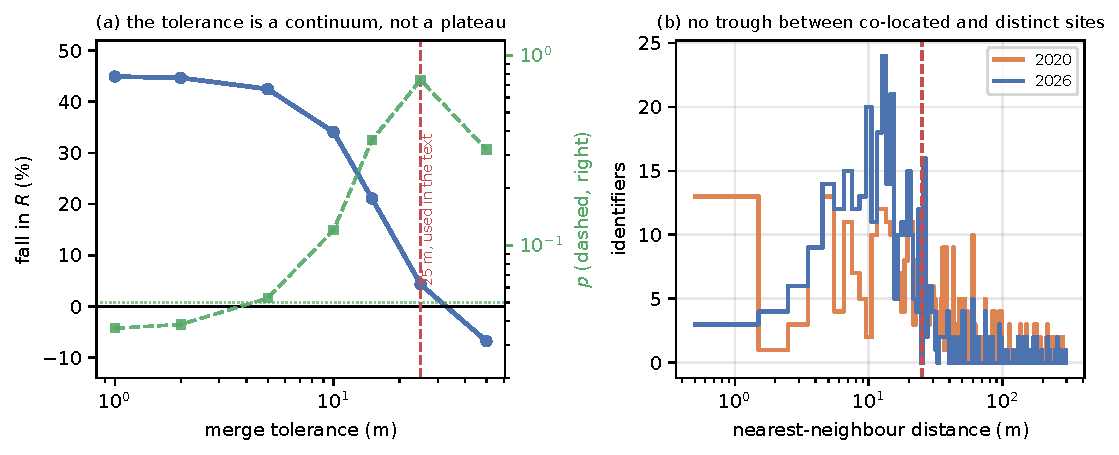
\includegraphics[width=0.99\textwidth]{figC8_tolerance.pdf}
\caption{The merge tolerance. (a) Fixed-hull $R$ and its OLS $p$-value against the merge radius; the dashed line is the \SI{25}{\meter} row of the tables. (b) Nearest-neighbour distances for 2020 and 2026.}
\label{fig:tolerance}
\end{figure}

\begin{figure}[htbp]
\centering
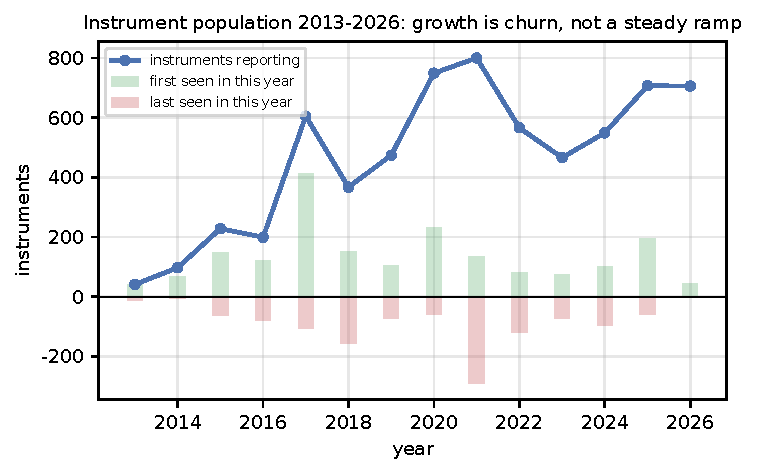
\includegraphics[width=0.92\textwidth]{figC1_population.pdf}
\caption{Instrument population, 2013--2026, with each instrument's first and last appearance.}
\label{fig:population}
\end{figure}

\subsection*{The apparent clustering trend is a measurement effect}
\label{sec:results-trend}

This is the paper's central result and it is negative. On the fixed-hull window, in
deduplicated locations, the Clark--Evans index falls from \rHullLocFirst{} in 2013 to
\rHullLocLast{} in 2026, a \locHullDrop\% reduction. The direction is the same under every
frame and unit, so it does not depend on that choice; the magnitude differs by more than
twenty points across them. We show that the fall is produced by three things that are not
geography --- densification, co-located registration, and the reference window --- and that once
all three are accounted for no trend in the nearest-neighbour geometry is detectable.
Figure~\ref{fig:clustering} gives the series on the fixed hull under both units.

\noindent\emph{The window.} $R$ scales as $A^{-1/2}$, so a smaller reference area \emph{raises}
$R$. The per-year bounding box moves by a factor of six across the record, so the box series is
moved by the window in both directions: the 2013 box is \SI{1056}{\kilo\meter\squared}, a quarter
of the hull, and the square root of the area ratio ($A_{\text{hull}}/A_{\text{box}} = 4.18$) is
$2.04$, which is the ratio of the two 2013 values (box $0.729$, hull $0.357$). By 2021 the box has
grown past the hull ($6489$ against \SI{4416}{\kilo\meter\squared}) and the box value is
\emph{below} the hull value. Quote either and the level is a property of the frame. We fix the
hull, which is the only frame on which the density denominator does not move, and report the box
beside it.

\noindent\emph{The window has a second form: the support mismatch.} The fixed hull is the union
of every year's points, and the early years occupy a small part of it --- the 2013 footprint is
\SI{671}{\kilo\meter\squared}, $0.15$ of the hull, and the 2021 footprint is $1.00$ of it
(Fig.~\ref{fig:study-area}b). Measured as bounding boxes, the 2013 network occupies
\SI{23.9}{\percent} of the reference frame and the 2026 network \SI{42.6}{\percent}. A
pattern confined to a fraction of its window has its $K$ inflated by roughly the inverse of that
fraction, so the early years carry a support penalty that the later years do not. Recomputing
every year on \emph{its own} hull, which matches the density denominator to the pattern's extent,
removes most of the decline: the \SI{1}{\kilo\meter} multiscale series becomes
$5505, 2598, 2291, 4364, \dots, 2114$ in place of $13640, 7673, 5251, 8991, \dots, 4028$, and its
fitted trend falls from \lKmExact{} m per year (se \num{110}) to \num{-99} m per year
(se \num{107}), which is not distinguishable from zero. The same defect therefore inflates the
box series in one direction and the fixed-hull series in the other, and neither is free of it.

\noindent\emph{The unit.} The exact-coordinate deduplication used above collapses only
identifiers at the \emph{same} coordinate; two registrations a few metres apart remain two
``locations''. Co-location is a property of the publishing schema, not of the deployment, and it
is large in the late years: \num{74.2}\% of 2026's identifiers have a neighbour within
\SI{25}{\meter} and \num{39}\% within \SI{5}{\meter}, against \num{9.8}\% in 2013. Merging
identifiers at that radius takes the fall to \num{4.3}\% (slope $+0.0014$, $p = 0.74$). The
result is monotone in the merge radius with no plateau, so the radius is a choice, not a
threshold the data identify: \num{\tolFallOne}\% at \SI{1}{\meter}, \num{\tolFallFive}\% at
\SI{5}{\meter}, \num{\tolFallTen}\% at \SI{10}{\meter}, \num{\tolFallFifteen}\% at
\SI{15}{\meter}, \num{4.3}\% at \SI{25}{\meter}, and \num{\tolFallFifty}\% --- a sign reversal
--- at \SI{50}{\meter} (Fig.~\ref{fig:tolerance}a; Table~\ref{tab:neardup}). What would justify a threshold is a trough
in the nearest-neighbour distribution separating co-located registrations from distinct
installations; there is none, the largest gap below \SI{200}{\meter} being \SI{\nnGapMax}{\meter}
in 2014 and \SIrange{6}{26}{\meter} in every other year, while the pooled distribution is smooth
across four orders of magnitude (Fig.~\ref{fig:tolerance}b). The merge is not an artefact of
the linkage rule either: complete-linkage gives \num{\clFall}\% ($p = \clP$), a centroid
representative gives \num{4.3}\%, and the largest cluster single-linkage forms has a diameter of
\SI{\chainMax}{\meter} against a median of \SI{\chainMedian}{\meter}, so chaining is bounded.
Grid-snapping instead gives \num{\gridSnapFall}\% ($p = \gridSnapP$), reported as a
limitation, not a footnote. Since the radius is not identified by the data, none of
these values has priority: they bound the effect, and do not estimate it.

\noindent\emph{The controls interact, so they do not decompose into shares.} It would be natural
to read the paragraphs above as three independent corrections and ask what fraction of the
\locHullDrop\% decline each accounts for. That reading is wrong, and the arithmetic says so. On
the fixed hull, merging at \SI{25}{\meter} removes the decline (\num{4.3}\%). But the support
correction goes the \emph{other} way: measuring each year on its own hull \emph{enlarges} the
decline to \rOwnHull\%, because a small early footprint raises the early-year index. Combine them
and the decline returns: on the merged unit and each year's own hull the fall is
\num{38.6}\% (slope \num{-0.0201}, $p = 0.004$). The four configurations are set out in
Table~\ref{tab:factorial}, together with the identifier baseline and the published-archive
figure they are measured from; they do not add up in any direction---one control removes the
effect and the other restores it. Registration and support are therefore reported as a
\emph{sensitivity range} (\locHullDrop\% down to \num{4.3}\% on the fixed hull, and
\rOwnHull\% under support matching), not as a partition. Equation~\eqref{eq:decomp} likewise
decomposes the \emph{index} into a distance term, a count term and a window term, and cannot
express the registration factor at all, since registration is not among its terms; it is an
identity, useful because it shows which term is on the right-hand side of the regression, not a
bookkeeping of the \locHullDrop\%.

\begin{table}[htbp]
\centering
\caption{The two controls in combination, on the location unit. They do not add up: registration alone removes the decline, and support matching restores it.}
\label{tab:factorial}
\footnotesize
\setlength{\tabcolsep}{5pt}
\begin{tabular}{llrrrr}
\toprule
Unit & Support window & Slope/yr & SE & OLS $p$ & Fall \\
\midrule
Identifiers (published) & fixed hull & $-0.0126$ & 0.0046 & 0.018 & 56.4\% \\
\textbf{Identifiers} & \textbf{fixed hull} & $\rHullSlope$ & \num{0.0046} & \hullIdsOlsP & \rHullDrop\% \\
Locations & fixed hull & \rHullLocSlope & \num{0.0046} & \hullLocOlsP & \locHullDrop\% \\
Merged \SI{25}{\meter} & fixed hull & $+0.0014$ & 0.0041 & 0.742 & 4.3\% \\
Merged \SI{25}{\meter} & own hull & $-0.0201$ & 0.0057 & 0.004 & 38.6\% \\
Exact locations & own hull & $-0.0382$ & 0.0059 & $<0.001$ & \rOwnHull\% \\
\bottomrule
\end{tabular}
\end{table}

\noindent\emph{The robust estimator sharpens the diagnosis and does not rescue the result.}
Replacing the mean nearest-neighbour distance with the median, against its own
complete-spatial-randomness expectation, gives a fall of \num{94}\%, against \num{45}\%. That
is the opposite of a rescue. A robust statistic that moves \emph{more} than the mean is telling
us the change lives in the body of the nearest-neighbour distribution, and for the late years
that body is the co-located mass. Under the merge the median behaves as the mean does
(\num{44.5}\% at \SI{25}{\meter}, $p = 0.32$), so it is not a substitute for the merged unit. We
report it as a diagnostic of where the change sits, not as a headline estimator.

\noindent\emph{Rarefaction.} Subsample every year to a common sample size and the trend
disappears: the rarefied location slope is \rRareLocSlope{} per year with a Newey--West interval
of $[\rRareLocLO, \rRareLocHI]$ containing zero, against \rHullLocSlope{} unrarefied. The null
is informative and not merely underpowered --- the minimum detectable effect at
\SI{80}{\percent} power is \rRareMDE{} per year, well below the unrarefied slope --- and an
equivalence test rejects at $p = \tostR$ within the unrarefied magnitude. Its limit must be
stated: with \rRareLocN{} locations the nearest-neighbour distance is set by separation at
kilometres, so the null rules out a coarse-scale trend and says nothing about the fine scale at
which the co-location operates. Table~\ref{tab:rare-r} gives the series year by year.

\begin{table}[htbp]
\centering
\caption{Clark--Evans $R$ on the fixed full-record hull, unrarefied and rarefied to a common sample size ($N = 41$ identifiers, $N = 39$ locations).}
\label{tab:rare-r}
\footnotesize
\setlength{\tabcolsep}{5pt}
\begin{tabular}{lrrrrr}
\toprule
 & & \multicolumn{2}{c}{Rarefied $R$} & \multicolumn{2}{c}{Unrarefied $R$} \\
\cmidrule(lr){3-4}\cmidrule(lr){5-6}
Year & $N$ (ids/locs) & Identifiers & Locations & Identifiers & Locations \\
\midrule
2013 & 41 / 39 & 0.357 & 0.367 & 0.357 & 0.367 \\
2017 & 605 / 518 & 0.369 & 0.391 & 0.233 & 0.258 \\
2021 & 800 / 729 & 0.461 & 0.466 & 0.407 & 0.429 \\
2026 & 706 / 561 & 0.352 & 0.382 & 0.155 & 0.202 \\
\bottomrule
\end{tabular}
\end{table}

\noindent\emph{The index identity, which is the cleanest quantitative result here.} On a fixed
frame
\begin{equation}
\ln R \;=\; \ln \bar{d} \;+\; \tfrac{1}{2}\ln N \;-\; \tfrac{1}{2}\ln A \;+\; \ln 2,
\label{eq:decomp}
\end{equation}
so the apparent trend in $R$ is the sum of a distance term, a count term and a window term. This
is an algebraic identity, not an allocation: it says which term of the index a regression moves,
and it has no registration term. We
verified the identity to $10^{-15}$ and fit the distance term directly. On the location unit
$\ln\bar{d} = \mathrm{const} + \hat\beta\ln N$ with $\hat\beta = \cleanSlopeLoc$
(se \cleanSELoc), against the $\beta = -\tfrac12$ that densification at constant shape forces:
the difference is \num{0.103}, $t = \cleanTLoc$, $p = \cleanPLoc$, so the densest years are
somewhat more clustered than density alone predicts but not significantly so. On the identifier
unit the same fit gives \cleanSlope{} (se $0.086$), $|t| = \cleanT$, which is the value the
published benchmark reports without naming the unit. On the merged unit the exponent
moves towards the structural value ($\cleanSlopeSite$ at \SI{10}{\meter},
$\cleanSlopeSiteTwo$ at \SI{25}{\meter}), the same registration effect appearing a third time.
Random thinning of the present pattern gives $\thinningBeta$ (se \num{0.066}) over twenty draws,
so the observed exponent lies between the densification value and the thinning value and is not
distinguishable from either. This exponent is the paper's one clean measurement and is not
attributed to a cause.

Two results here are established, not asserted. \emph{Registration}, not geography, produces
the co-location, and the archive itself says so: the collapse is confined to one of the two
published coordinate resolutions and is unchanged when the other is rounded to the same quantum,
so the co-located records are duplicated registrations, not positions quantised into
coincidence (the co-location analysis). \emph{The apparent clustering trend}, once that
and the window are controlled, leaves no trend in the nearest-neighbour geometry
(the clustering-trend analysis). The first names a cause for the measurement effect; the second
removes it from the geography. We do not extend that cause to the deployment.

\subsection*{The unit of analysis, and the concentration index}
\label{sec:results-unit}

Co-located identifiers are an artefact of the publishing schema, not of geography, and
removing them changes the headline, so the location is the headline unit and the identifier
figure is reported beside it. Of the \nAnalysed{} identifiers that enter the spatial analysis,
\nLocations{} occupy distinct coordinates; \nShared{} of them, or \sharePct\% of the population,
sit at a coordinate another identifier also occupies, and the surplus is \nSurplus{} or
\surplusPct\%. The identifier series is not wrong to report --- it is what the platform counts
--- but it double-counts the schema, so it is the secondary figure. \emph{Concentration is a
sample-size effect in the same way.} The Gini of occupied cells rises at $\giniRawSlope$ per
year uncorrected, and rarefying every year to a common sample size reverses the sign
($\giniRareSlope$ at 20 cells per side; \num{-0.0068}, \num{-0.0106} and \num{-0.0076} at 30,
40 and 50). The two answers are of opposite sign and neither is negligible, so the index does
not identify a direction of change, and at fine resolutions it is near-degenerate --- at 50
cells per side the smallest sample occupies 24 of 2500 cells and most counts equal one. No
claim about concentration is made in either direction. The grid resolution, grid origin, gap
filled roster and core-definition sweeps are in the Supplemental Information.

\begin{table}[htbp]
\centering
\caption{The fixed-hull location series under tolerance deduplication: single-linkage at radius $r$, one identifier kept per cluster. The published row clusters at $r = \SI{1}{\milli\meter}$, the finest distinction the projected coordinates carry, so its counts differ from the \num{561} locations of Table~\ref{tab:summary} by the millimetre-scale pairs that survive there and collapse here; the trend is the same either way (slope \num{-0.0107} to \num{-0.0108} per year, $p = 0.035$ to $0.037$, a \num{45.0} to \num{45.3}\% fall).}
\label{tab:neardup}
\footnotesize
\setlength{\tabcolsep}{5pt}
\begin{tabular}{lrrrrrr}
\toprule
Deduplication & 2013 $R$ & 2026 $R$ & Fall & Slope/yr & OLS $p$ & 2026 $z$ \\
\midrule
Exact coordinate (published) & 0.367 & 0.201 & 45.3\% & $-0.0108$ & 0.035 & $-6.6$ \\
Within \SI{5}{\meter}         & 0.367 & 0.211 & 42.5\% & $-0.0101$ & 0.053 & $-6.8$ \\
Within \SI{10}{\meter}        & 0.367 & 0.242 & 34.1\% & $-0.0076$ & 0.120 & $-6.0$ \\
Within \SI{25}{\meter}        & 0.367 & 0.351 & 4.3\%  & $+0.0014$ & 0.742 & $-3.6$ \\
\bottomrule
\end{tabular}
\end{table}

\begin{figure}[htbp]
\centering
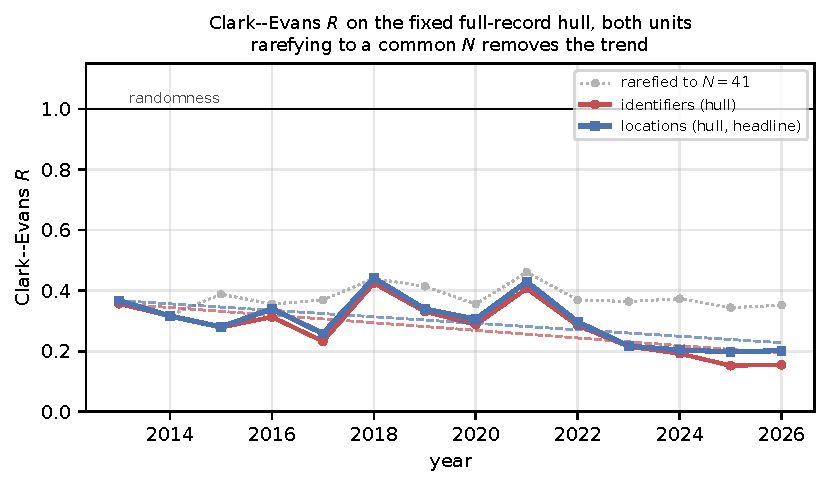
\includegraphics[width=0.92\textwidth]{figC2_clustering.pdf}
\caption{Clark--Evans $R$ by year on the fixed full-record hull, both units, with the rarefied series and the fitted trends. The band is the homogeneous CSR envelope.}
\label{fig:clustering}
\end{figure}

\begin{figure}[htbp]
\centering
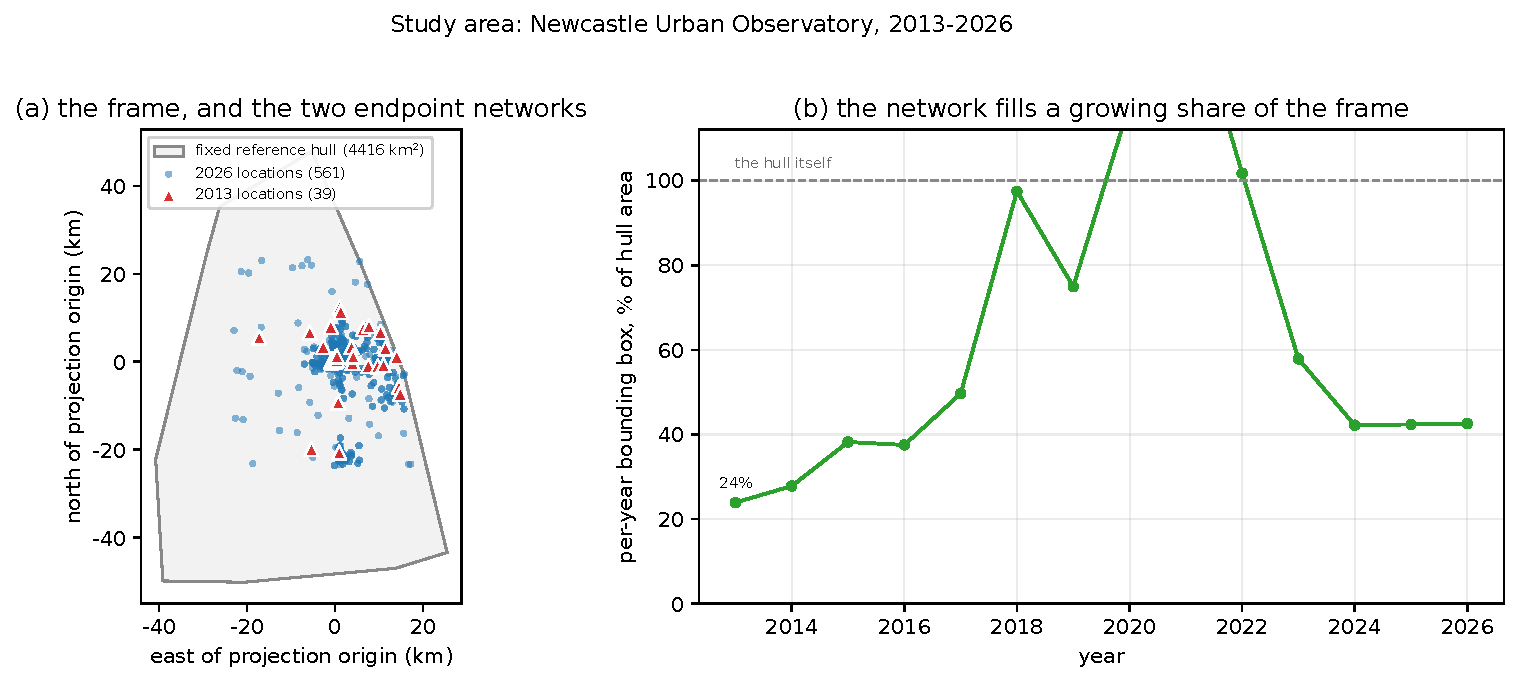
\includegraphics[width=0.98\textwidth]{figC0_study_area.pdf}
\caption{The study area. (a) The fixed reference hull, with the 2013 and 2026 networks on it. (b) Each year's bounding box as a share of that hull.}
\label{fig:study-area}
\end{figure}

\subsection*{The co-location is duplicated registration, not a rounding artefact}
\label{sec:results-origin}

The merge radius would be a free choice only if the co-location had no origin we can identify.
It has one, and the archive records it. Coordinates are published to two different resolutions:
\num{36.8}\% of identifier--year records are written to six decimal places or fewer, a quantum of
about \SI{0.11}{\meter} in latitude, and \num{42.8}\% to twelve places or more, where the printed
value is sub-millimetre. These are two publishing paths, not two kinds of instrument. The
remaining \num{20.5}\% sit between seven and eleven places and belong to neither class, so this is
a description of the two dominant paths and not a partition of the record; Table~\ref{tab:precision}
counts the two classes only, which is why its annual totals fall below the identifier count.

Pooled over the record, \num{62.5}\% of high-precision records have a neighbour within
\SI{25}{\meter} against \num{32.6}\% of low-precision records, so co-location is roughly twice as
common where coordinates are published at full resolution. The comparison does not hold in that
direction for every year. In the later years it inverts: on the sub-metre scale, \num{73.2}\% of
low-precision records in 2026 have a neighbour within \SI{0.5}{\meter} against \num{8.3}\% of
high-precision records, the reverse of the pooled reading. The two classes therefore do not
differ by a constant factor; whichever path co-locates changes over the record, and the merge
tolerance crosses that change instead of sitting on one side of it.

What survives all of this is a narrower statement, and it is the one that identifies the origin.
Rounding the high-precision class to the low-precision quantum leaves its co-location unchanged:
2017 stays at \num{17.3}\% and 2020 at \num{14.8}\%, while the same years' low-precision class
sits at \num{3.8}\% and \num{0.9}\% (Table~\ref{tab:precision}). The co-located pairs are
therefore already coincident to better than a tenth of a metre, in the class where rounding could
not have created them. The co-location is duplicated registration in the archive, not
precision lost in publication.

It also survives inside one class, but only weakly, and the qualification matters. Restricting to
high-precision records only and holding the sample size fixed at \num{33} by random subsampling
over the eleven years for which that class is populated, the fall is \num{34.3}\%. The matched
control --- random subsets of the pooled high-precision locations at the same size --- has a mean
fall of \num{8.1}\% with a \SI{95}{\percent} interval of $[-56.0, 56.8]$ over \num{200} draws.
The observed \num{34.3}\% therefore lies \emph{inside} that interval: it sits at the
\num{84.5}th percentile of the control distribution, which is suggestive but not significant at
the \SI{5}{\percent} level. We report it as consistent with one path carrying part of the effect
without the mixing of two paths, not as an independent confirmation of it, because the interval
that would have to be excluded spans both signs.

The collapse is not uniform across years, and it follows registration, not geometry. In
2025 and 2026 the low-precision class collapses to \num{43.6}\% and \num{44.7}\% while the
high-precision class sits at \num{9.1}\% and \num{3.6}\%; in 2017 and 2021 the ordering reverses,
the high-precision class at \num{17.3}\% and \num{14.9}\% against \num{3.8}\% and \num{0.3}\%.
The identity of the co-locating path therefore changes across the record, and the merge tolerance
crosses that change. This is why the curve has no plateau. The radius is not locating a physical
separation between co-located and distinct installations; it is progressively removing whichever
path co-locates first, and the path that does so is not the same one throughout. The
\SI{25}{\meter} value is the smallest radius at which neither path shows a substantial collapse,
and it is a bound on the artefact, not a measurement of the deployment.

\begin{table}[htbp]
\centering
\caption{Exact-coordinate collapse by published coordinate precision, 2017--2026. Rounding the high-precision records to the low-precision quantum (\SI{0.11}{\meter}) leaves the value unchanged, so the co-location is duplicated registration.}
\label{tab:precision}
\footnotesize
\setlength{\tabcolsep}{5pt}
\begin{tabular}{lrrrr}
\toprule
 & \multicolumn{2}{c}{High precision (12 or more dp)} & \multicolumn{2}{c}{Low precision (6 or fewer dp)} \\
\cmidrule(lr){2-3}\cmidrule(lr){4-5}
Year & $N$ & Collapse & $N$ & Collapse \\
\midrule
2017 & 283 & 17.3\% & 182 & \phantom{0}3.8\% \\
2020 & 317 & 14.8\% & 320 & \phantom{0}0.9\% \\
2021 & 343 & 14.9\% & 374 & \phantom{0}0.3\% \\
2025 & 350 & \phantom{0}9.1\% & 257 & 43.6\% \\
2026 & 336 & \phantom{0}3.6\% & 284 & 44.7\% \\
\bottomrule
\end{tabular}
\end{table}

\subsection*{What survives: a multiscale level, not a trend}
\label{sec:results-mech}

Against an \emph{inhomogeneous} null that preserves each year's first-order intensity --- a
kernel-smoothed surface fitted to that year's own points and resampled \num{199} times, with the
\SI{750}{\meter} bandwidth stated because the result depends on it --- the multiscale function
$L(r)$ exceeds the entire envelope at \SI{250}{\meter} to \SI{1.5}{\kilo\meter} in all fourteen
years, at \SI{100}{\meter} in thirteen (the exception being 2013, whose \dropNt{} locations
cannot resolve that scale) and at \SI{2}{\kilo\meter} in twelve, and it never falls below it at
any scale in any year. That is a stronger statement than the single-index version of the same
test, because $L$ uses the border-corrected estimator and the location unit removes the co-located channels.
The surface is fitted to the points it tests, so the separation is a description, and the
scale range over which it is unanimous is stated.

Its \emph{decline}, however, does not survive support matching, as
the clustering-trend analysis shows. Note first that this fall is not the same movement as the
one in the nearest-neighbour index, and the two are worth naming separately because they run in
opposite directions at their own scales. A \emph{falling} $R$ means nearest neighbours sit
closer than the density predicts, that is \emph{more} short-range clustering; a \emph{falling}
$L$ at \SI{1}{\kilo\meter} means fewer excess neighbours at that scale, that is \emph{less}
medium-scale clustering. The two indices are therefore not two readings of one change, and
this paper's subject is the apparent strengthening of the \emph{nearest-neighbour} geometry,
which is the index that does not survive. Wherever this paper says ``the decline'' without naming
an index, $R$ is meant.

What survives for $L$ is not a trend but a level: on
footprint-matched windows the 2013 network is more clustered at \SI{1}{\kilo\meter}
(\num{5505} m) than the present network is inside the same footprint at the same density
(envelope \num{502}--\num{1986} m), and nine of the eleven testable years lie above their own
envelope. The early network differs from the present one at medium scales; the record does not
show a continuing drift, and the fitted slope halves when 2013 is removed
($-269$ m per year, $p = 0.019$, against \lKmExact{} over all years). The footprint-matched
procedure is defined in the estimator section and tabulated in the Supplemental Information:
for each year, the present network's locations that fall inside that year's own convex hull are
compared with the multiscale function of the year's own points at the same density, so the window
and the sample size are held to the year being judged.

\subsection*{Size and time cannot be separated, and the infill question is open}
\label{sec:results-powerlaw}

The association between clustering and size looks strong on the per-year window
($\ln R = 1.163 - 0.369\ln N$, $R^2 = 0.849$) and does not survive fixing the window: at a fixed
area the size term is dominated by the identity of Equation~\eqref{eq:decomp}, the exponent is
not distinguishable from the structural value, and the rarefied series has no time trend
either --- subject to the scale limit stated where rarefaction is introduced, that at
\rRareLocN{} locations it resolves only structure above about \SI{5}{\kilo\meter}, so it
excludes a coarse-scale time trend and not a fine-scale one.
Neither size nor elapsed time is identified, so the change is attributed to neither.

One diagnostic that might have attributed it does not. If new instruments filled the gaps
\emph{between} existing ones, the network would be densifying inward; if they arrived outside,
it would be expanding. We tested this by pooling each year pair's locations and permuting the
new/existing labels, which holds the spatial support and the intensity fixed. On the published
unit new locations lie \emph{further} from the existing set than the permutation holds, in
\rlAbove{} of \rlPairs{} year pairs, and they also cluster among themselves relative to a
pooled-subset null in \batchPairs{} of \batchTotal{} pairs --- consistent both with outward
expansion and with batches deployed into contiguous new ground, which this record cannot
separate. Both counts halve once co-located registrations are merged (\num{7} of \num{13} and
\num{6} of \num{13}), so even this diagnostic is a statement about the published unit. We
therefore report no mechanism.

\subsection*{Two publication discontinuities}
\label{sec:results-theme}

The platform changed what it published twice, and both changes are visible in the archive rather
than in the city. Vehicle share collapses to 16.8\% in 2018 on identifiers (17.4\% on locations)
because the vehicle files for 2017 carry \texttt{Cars} and \texttt{Parking~Spaces} and the 2018
files do not; a reader using 2018 as representative of that theme would be reading the
publishing schema. Archive file counts run 11--75 per year to 2025 and then jump to \textbf{257}
in 2026, when the platform began publishing monthly files, not bundled ones, while the
instrument roster is continuous (706 against 707), so the discontinuity is in file granularity
and not in the deployment. Neither propagates into the fitted trend: on the fixed hull the slope
moves from $-0.011$ to $-0.010$ across the four exclusion samples, a range of $0.0011$ against an
interval of $0.016$ for those coefficients, and on the box frame it is unchanged to within 8\%.
The final year covers nine months, not twelve, and every headline result is reported with
and without it: dropping it leaves the permutation test marginal ($p = \hullNoLastPermP$) while
Mann--Kendall, which depends on rank order, not year values, still rejects
($p = \hullNoLastMkP$), so the decline is better described as monotone than as linear. The theme
composition, the gap-filled roster, the core sweep and the exclusion sweeps are in the
Supplemental Information.

\section*{Discussion}
\label{sec:discussion}

\subsection*{What this means for anyone using this network}
\label{sec:disc-longitudinal}

A study that uses this observatory at a single moment is using one geometry from a series whose
size grew \growth$\times$ and whose apparent clustering fell by between 4.3\,\% and 67\,\%
depending on how co-located registrations are counted and which window is used. The practical
warning is therefore not a number but the dependence itself: a spatial result computed against
this platform is conditioned on the year, the frame and the unit, and that conditioning is not
usually reported. The same caution applies to derived products built on open platform data,
including the interoperability layers and digital-twin interfaces that aggregate a platform
without re-censusing it \citep{anthony2024enabling}, and to the frozen snapshots used as
execution targets; one such snapshot is audited here, and the audit is in the Supplementary
Material. This is the same family of problem \citet{xia2026measurement} identify for carbon inventories: an apparent structural property
that depends on how the measurement was constructed. Their construction variable is accounting
choice; ours is the definition of the unit and the frame.

\subsection*{A transferable rule for longitudinal spatial reporting}
\label{sec:disc-transfer}

The specific numbers above belong to one city. The argument that produced them does not, and
this is the part of the paper we expect to outlive the case. Wherever a sensor platform
re-registers instruments under new identifiers, and wherever a longitudinal study reads a
density-dependent spatial index, the same three quantities condition the answer, and each can be
reported at no cost to the analysis:

\begin{enumerate}
\item \textbf{The support of each year's pattern, beside the window it is measured in.} A window
inherited from the union of the record penalises its early years by a factor near the inverse of
the area they occupy --- here $0.15$ of the hull in 2013 --- and inflates them in the other
direction as the window is fixed. Reporting the occupied area per year makes the penalty visible;
measuring on each year's own footprint removes it.
\item \textbf{The degree of registration co-location, as a distribution, not a flag.} The
share of identifiers with a neighbour inside a stated radius suffices, reported per year. One
number states the problem and its growth; a binary ``deduplicated'' flag hides both, and cannot
distinguish an archive that is clean from one where co-location arrived with a schema change.
Where the archive publishes coordinates at more than one resolution, the share should be reported
\emph{per resolution}, because the classes need not co-locate alike and here they do not: one path
collapses to \num{44.7}\% while the other sits at \num{3.6}\% in the same year. That single
split is what identifies the artefact as duplication, not geometry, and it is available
before any clustering is computed.
\item \textbf{The rarefied and unrarefied series together.} A count-based index confounds a
change in arrangement with a change in population, and the two answers can carry opposite signs,
as they do for the concentration index here. Reporting both separates a genuine rearrangement
from a sample-size effect.
\end{enumerate}

None of the three requires a new estimator, a model, or a judgement about the deployment, and
together they convert an unreportable conditioning into a stated one. The broader point is that
for a growing sensor network the measurement protocol is not fixed while the object changes; the
window, the sample size and the identity of the unit all move with the network, so a longitudinal
statistic is stable only if those three are held and reported. That claim is independent of this
city, and it is the reason the factorial comparison in the clustering-trend analysis is worth
performing, not the trend worth quoting.

\noindent\emph{The headline is a floor on the measurement effect, not a ceiling.} The
\locHullDrop\% decline is measured on a window fixed across years. Measuring each year on its own
hull instead \emph{enlarges} it to \rOwnHull\% (\rOwnHullFirst{} to \rOwnHullLast), because a
small early footprint raises the early-year index: $R$ scales as $A^{-1/2}$, so the 2013 network's
\SI{671}{\kilo\meter\squared} footprint lifts its index well above its fixed-hull value. Support
matching and the per-year box therefore both move in the same direction, and the fixed hull is the
conservative choice. An earlier version of this paper described the fixed-hull figure as an upper
bound set jointly by the three factors; that description was wrong in direction and is corrected
here. What the three factors do is reduce the decline when they are controlled one at a time
(registration to \num{4.3}\%, the support-matched multiscale slope to zero), not bound it from
above.

\subsection*{Limitations}
\label{sec:limits}

The record has fourteen annual points with size and year collinear, so nothing here is an
attribution. Five further limits bear on specific claims. \emph{The merge tolerance is not
identified by the data} (the clustering-trend analysis), so the effect is bounded, not
estimated, and grid-snapping gives a different answer again ($\num{\gridSnapFall}\%$). \emph{The
rarefied null} resolves only structure above about \SI{5}{\kilo\meter}, so it rules out a
coarse-scale time trend and says nothing about the fine scale at which the co-location operates.
\emph{The window is not neutral}: the fixed hull is the union of every year's points, so a few
outlying sites set the denominator for all years, and the earliest years carry a support penalty
from which no density-dependent index is free. \emph{The HAC intervals are anti-conservative at
this length}: simulated on pure noise at fourteen points the OLS-plus-Newey--West test rejects at
a nominal \SI{5}{\percent} about \nwSize\% of the time, rising to \nwSizeAr\% at the lag-1
residual autocorrelation the headline series actually shows ($+0.15$) and \nwSizeArHigh\% at
$\rho = 0.5$. The plain OLS test is a different case and the distinction matters: it is correctly
sized in the same simulation, rejecting \SI{\olsSizeIid}{\percent} under independent errors, and
mildly optimistic at the series' own autocorrelation
(\SI{\olsSizeAr}{\percent}). So the fixed-hull $p$-values are neither safely conservative nor
badly inflated, and we carry each claim on more than one procedure rather than treating any
single $p$-value as calibrated.
\emph{The concentration index
of occupied cells is not usable at fine resolutions}: rarefied, it is negative at every
resolution with a rank interval excluding zero while the uncorrected series is positive, so
rarefaction reverses its sign, and at 50 cells per side the smallest sample occupies 24 of 2500
cells, so most counts are one. Concentration is unresolved in either direction.
The thematic composition, the gap-filled roster and the core-definition sweep are sensitivities
in the Supplemental Information, and none of them changes a conclusion above.

\section*{Conclusions}
\label{sec:conclusions}

We set out to ask how much of the apparent strengthening of clustering in the Newcastle Urban
Observatory is a property of the deployment, not of the measurement. Conditional on the merge
tolerance the answer is: almost none of it. On the exact-coordinate unit that the paper leads
with, and on a window fixed across years, the Clark--Evans index falls \locHullDrop\%. Merging
registrations within \SI{25}{\meter} --- a radius the data do not identify, so that figure is a
bound and not an estimate --- leaves \num{4.3}\%, monotonically in the radius and with no
plateau. The honest reading is therefore a range rather than a point, and a reader who takes
co-located registrations to be one instrument should read the decline as small.

No part of the \locHullDrop\% is geography that has been shown to move. The
reference window moves the level in both directions and has a second form as a support mismatch
between the early footprints and the window they are measured in, which \emph{enlarges} the
decline to \rOwnHull\% rather than reducing it; the count term is on the
right-hand side of the index by construction; and co-located registration, which is a property of
how the platform records instruments, removes the decline outright. The three do not partition
the \locHullDrop\% into shares, and we do not present them that way: they interact, and
registration and support matching pull in opposite directions
(Table~\ref{tab:factorial}). What the combination establishes is that there is no version of the
measurement, on any unit or window we tested, in which most of the \locHullDrop\% is left as
geography once registration is controlled. Once all three are
controlled, no trend in the nearest-neighbour geometry is detectable: rarefaction to a common
sample size removes it, and the mean nearest-neighbour distance scales with population at
$\cleanSlopeLoc$ (se \cleanSELoc), not distinguishable from the $-\tfrac12$ that densification
at constant shape forces. The multiscale decline is largely a support artefact as well,
falling from \lKmExact{} to \num{-99} m per year when each year is measured on its own
footprint.

What survives is smaller than the headline, and it is the residual. The network is
clustered relative to its own smoothed intensity at \SI{250}{\meter} to \SI{1.5}{\kilo\meter} in
all fourteen years, and it was more clustered at \SI{1}{\kilo\meter} in 2013 than the present
network is inside the same footprint at the same density --- a level difference, not a
trend, since the fitted slope halves once 2013 is removed. Membership turns over continuously
and does not accumulate, at a median replacement rate of \replMedian{}, and that is the one
result here not conditioned on the unit or the frame. Size and elapsed time cannot be separated
at fourteen collinear points, so the exponent is the paper's one clean measurement and is
attributed to neither.

Three consequences follow. For users of this network, the year of analysis is a conditioning
variable that should be reported alongside any spatial result, and a registration rule that
merges co-located channels is a reporting decision, not a preprocessing detail. That
conditioning is not peculiar to this platform, and the reporting rule it implies is set out in
the transferable rule: report the support of each year's pattern beside its window, the
degree of registration co-location as a distribution, not a flag, and the rarefied series
beside the unrarefied one. For those
building longitudinal urban sensing datasets, births and last appearances are more informative
than a net instrument count. And a frozen snapshot used as an execution target should carry a
provenance statement, because the snapshot audited here covers \covPct\% of the instruments that ever
reported and omits vehicle counters, at an odds ratio of \snapCondOR{} when the comparison is
conditioned on the snapshot's own year.
















\section*{Acknowledgments}
\noindent The Newcastle Urban Observatory at Newcastle University is credited for maintaining an open, long-running municipal data platform; a census of this kind is only possible because the data are published without restriction.

\section*{Additional Information and Declarations}

\subsection*{Funding}
\noindent This research work was funded by Umm Al-Qura University, Saudi Arabia under
grant number: \uquGrant{}.

\subsection*{Grant Disclosures}
\noindent The following grant information was disclosed by the author: Umm Al-Qura University (Deanship of Postgraduate Studies and Scientific Research), 26UQU4350624GSSR07.

\subsection*{Competing Interests}
\noindent The authors prepared the benchmarking artifact whose provenance this
paper audits, so the authors have a non-financial interest in the audit it receives; the audit
is disclosed both in that section and here so that a reader can weight it. Apart from that, the
authors declare no competing interests. The Newcastle Urban Observatory data the artifact
derives from are independently published by \citet{uo_archive}.

\subsection*{Author Contributions}
\noindent \noindent Ammar Arbaaeen: Funding acquisition, Writing -- review and editing. Wael Alnahari: Conceptualization, Methodology, Software, Validation, Formal analysis, Data curation, Writing -- original draft, Writing -- review and editing, Visualization, Project administration. Tawfiq Hasanin: Validation, Writing -- review and editing. Ammar Alsaig: Writing -- review and editing. Wasem Alnahri: Conceptualization, Validation, Writing -- review and editing.

\subsection*{Data Availability}
\noindent The source data are the Newcastle Urban Observatory collection, openly
archived by Newcastle University under CC BY 4.0 \citep{uo_archive}. The derived census,
the fitted models, the snapshot audit and every analysis script behind the numbers in this
paper are openly archived under CC BY 4.0 at
\url{https://doi.org/10.5281/zenodo.23099939}, which always resolves to the current version,
and are also provided as Supplemental Information. The deposit also carries the benchmark
snapshot itself, the one-week instrument catalogue the snapshot audit is computed from, so
that audit can be re-run from the deposit alone. That catalogue is a list of instruments ---
identity, position, broker and variable names --- and every measured quantity in it has been
removed; no temperature, concentration or count is redistributed, and none is read by any
analysis. The deposit contains no observatory observations and no credential: what is
deposited is our own work \emph{about} the collection, together with the record of which
instruments it was computed over. Related work on query
performance over this platform is documented separately \citep{alnahari2026complexity}.

\subsection*{Supplemental Information}
\noindent Supplemental Information S1. Supporting material: the annual census and fitted models, the
snapshot audit, and the analysis scripts that produce every number and figure in this
paper.

\subsection*{Notes on contributors}
\noindent \textbf{Ammar Arbaaeen} and \textbf{Ammar Alsaig} are in the Department of Computer Science, College of Computer and Information Systems, Umm Al-Qura University, Saudi Arabia. \textbf{Wael Alnahari} is in the Department of Information Systems, Faculty of Computing and Information Technology, King Abdulaziz University, Saudi Arabia. \textbf{Tawfiq Hasanin} is in the Department of Information Systems, King Abdulaziz University, Saudi Arabia. \textbf{Wasem Alnahri} is an independent researcher, Saudi Arabia.

\subsection*{Generative AI Use Disclosure Statement}
\noindent \textbf{Tool and version.} Tool: GitHub Copilot, version 0.69.0. \textbf{How it was used.} Drafting and editing LaTeX and typesetting support. \textbf{Reason for use.} Assistance with manuscript preparation and language. It was not used to compute, alter or select any result; every number in the manuscript is read from a committed results file produced by the analysis scripts in the deposit. \textbf{Originality and accuracy.} The authors confirm the originality and accuracy of the content. \textbf{Terms of use.} The authors have checked the terms of use for this tool and confirm its use is suitable for publication. \textbf{Responsibility.} The authors take full responsibility for the integrity of the whole content, including the accuracy of all references.


\bibliography{references}

\end{document}
